%
% ─── CAPITULO 8: VISUALIZACION DE FRACTALES 3D ──────────────────────────────────
%

En el capítulo \ref{chap:fractales-2D} introdujimos técnicas y código necesario para poder visualizar conjuntos de Julia y conjuntos de Mandelbrot 2-dimensionales en un canvas utilizando WebGL, todo ello apoyado en la teoría explicada en el capítulo \ref{chap:Julia-Mandelbrot}. Sin embargo, el objetivo de éste y de los tres capítulos anteriores es aplicar técnicas avanzadas de cálculo de imágenes para poder visualizar fractales en tres dimensiones. Recordamos que explicamos en la introducción del capítulo \ref{chap:ray-tracing} que la mejor forma de generar imágenes de fractales 3D es utilizando la técnica de `Ray Tracing', que en dicho capítulo explicamos con detalle. A pesar de ello y de conseguir escenas con varios objetos, materiales y movimientos de cámara no visualizamos nada lejanamente parecido a un fractal. Será en este capítulo en el que aprovecharemos toda la infraestructura y todo el código implementado hasta el momento en el `ray-tracer' del capítulo \ref{chap:ray-tracing} para graficar fractales tridimensionales.

Para ello, antes aún debemos asentar una serie de conceptos que son los que nos ayudarán a cumplir nuestro objetivo: el algoritmo \textit{Ray-Marching} y las conocidas como \textit{Signed Distance Functions} (SDFs). Con estos dos elementos combinados conseguiremos ver hermosas figuras fractales.

\section{El algoritmo Sphere-Tracing}
\label{section:sphere-tracing}

Hasta ahora siempre hemos calculado las intersecciones rayo-esfera de manera totalmente analítica, ya que es muy sencillo describir una esfera o un plano mediante una ecuación y solucionar esta ecuación en $t$, como vimos en las secciones \ref{subsection:esfera} y \ref{subsection:plano}. Sin embargo, no es tan sencillo encontrar ecuaciones que describan la superficie de los fractales. Es por esto que necesitamos otra manera de encontrar las intersecciones rayo-superficie. Recordemos entonces que en la sección \ref{section:elementos-RT} hablamos de que además de las expresiones analíticas las intersecciones se pueden calcular mediante métodos iterativos. 

En literatura, se denomina \textit{Ray-Marching} a cualquier método numérico iterativo utilizado para encontrar intersecciones mediante movimientos a lo largo de un rayo. Sobre este tema hay mucha literatura y es un tema de interés vigente. El método más sencillo es la búsqueda de raíces de una función mediante el método de Newton generalizado a $\R^3$, pero existen técnicas más avanzadas. 

El algoritmo \textit{Sphere-Tracing} es una de estas técnicas de ray-marching descrita por \textit{John C. Hart} en \cite{Hart-1995}. Se basa estimar la distancia más corta de un punto en el rayo a cada una de las superficies que componen la escena, identificar la mínima de estas y avanzar en el rayo dicha distancia, pues se tiene la certeza de que al menos en una esfera de radio dicha distancia no hay ninguna intersección con ningún otro cuerpo. Una vez se ha avanzado en el rayo se repite esta operación y así sucesivamente hasta que la estimación de la distancia mínima es lo suficientemente pequeña como para considerar que el punto forma parte de una superficie.

Aclaramos que \textit{Ray-Marching} y \textit{Sphere-Tracing} no son sinónimos, aunque en ocasiones se abusa del lenguaje y se utilizan indistintamente. Sphere-Tracing es un tipo de técnica de Ray-Marching, siendo este último un concepto que engloba no solo a sphere-tracing, sino a toda técnica iterativa que busque intersecciones recorriendo el rayo.

Pongamos un ejemplo. Supongamos que tenemos una escena con una esfera tangente al plano horizontal $y=0$, un rayo $R$ fijo y queremos aplicar Sphere-Tracing para encontrar la intersección.

\begin{figure} [ht]
    \centering
    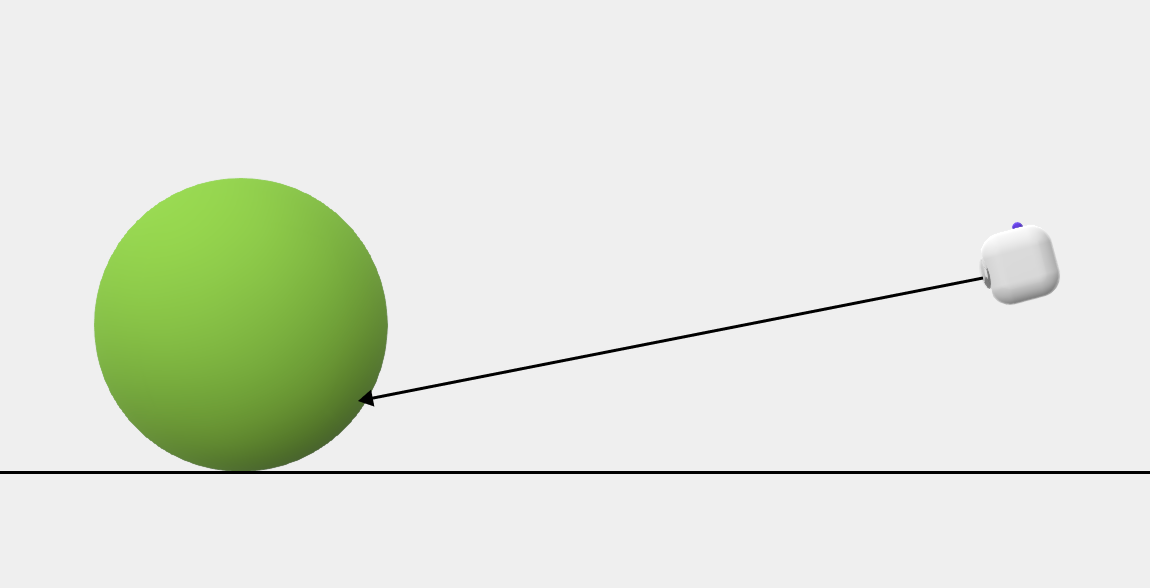
\includegraphics[scale = 0.2]{img/C8/situacion-inicial.png}
    \caption{Situación a la que aplicar Sphere-Tracing}
    \label{fig:ST-inicial}
\end{figure}

La distancia de un punto $p$ a una esfera $S$ de centro $c$ y radio $r$ es 
\begin{equation}
    \label{eq:distancia-punto-esfera}
    d(p,S) = \|p-c\| - r 
\end{equation}
y la distancia de un punto al plano $y=0$ es simplemente su componente $y$. Por tanto, partiendo del origen, calculamos la distancia a la esfera y la distancia al plano, vemos que es menor la del plano, por lo que avanzamos en el rayo una distancia igual a la calculada para el plano (imagen \ref{fig:iteraciones-ST} (a)). Seguidamente repetimos la operación: volvemos a calcular la distancia a la esfera y al plano. De nuevo el plano es el objeto más cercano, por lo que avanzamos en el rayo la misma distancia que había hasta el plano (imagen \ref{fig:iteraciones-ST} (b)).

\begin{figure}[ht]
    \centering
    \begin{tabular}{ccc}
      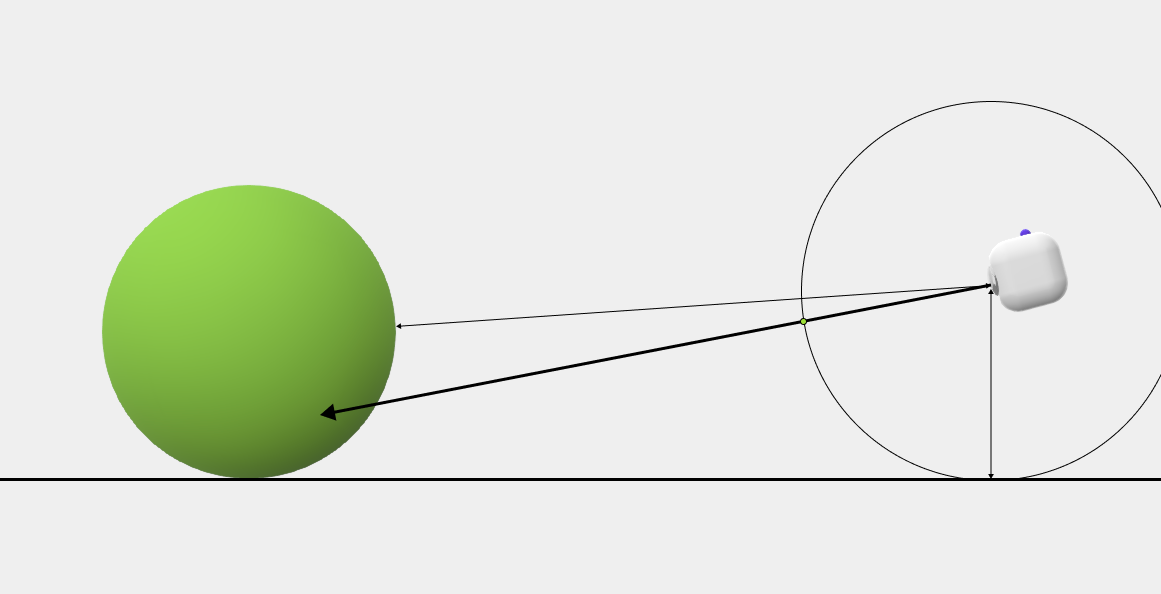
\includegraphics[scale=0.16]{img/C8/sphere-tracing-1.png} &     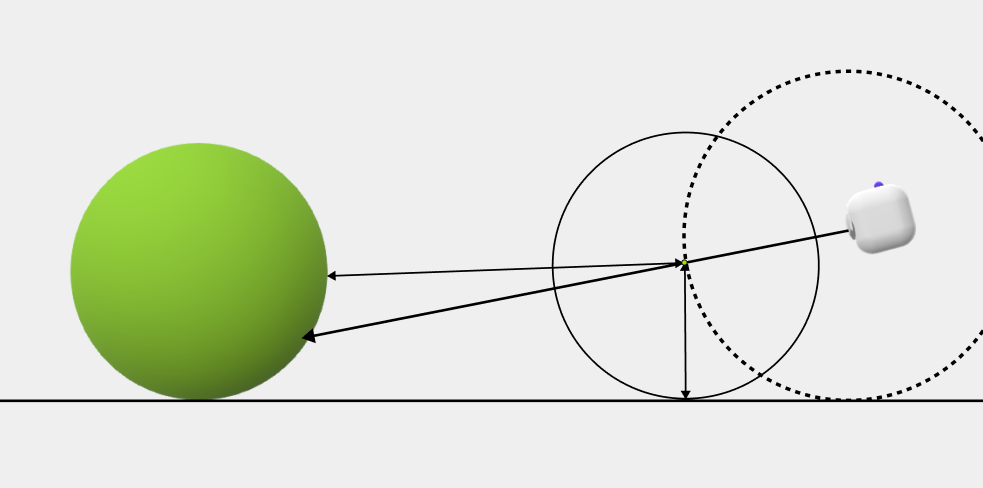
\includegraphics[scale=0.196]{img/C8/sphere-tracing-2.png} \\
    (a) Primera iteración & (b) Segunda iteración \\[6pt]
    \end{tabular}
    \caption{Dos primeras iteraciones de Sphere-Tracing}
    \label{fig:iteraciones-ST}
\end{figure}

Si repetimos este proceso indefinidamente, llegará el momento en el que la distancia a la esfera será tan pequeña que consideraremos que el punto está en la esfera y habremos encontrado la intersección (imagen \ref{fig:finales} (a)). En caso de que no exista ninguna intersección, el algoritmo seguirá avanzando en el rayo, pero al no encontrar nunca una distancia suficientemente pequeña se avanzará indefinidamente (imagen \ref{fig:finales} (b)), por lo que hay que fijar una distancia máxima recorrida y/o un número máximo de iteraciones como parámetro del algoritmo.

\begin{figure}[ht]
    \centering
    \begin{tabular}{ccc}
      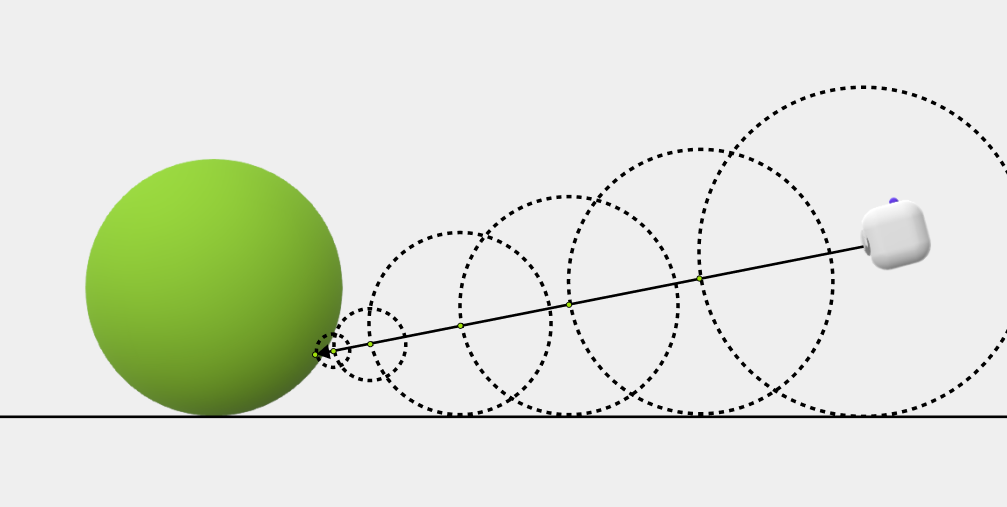
\includegraphics[scale=0.2]{img/C8/sphere-tracing-final.png} &     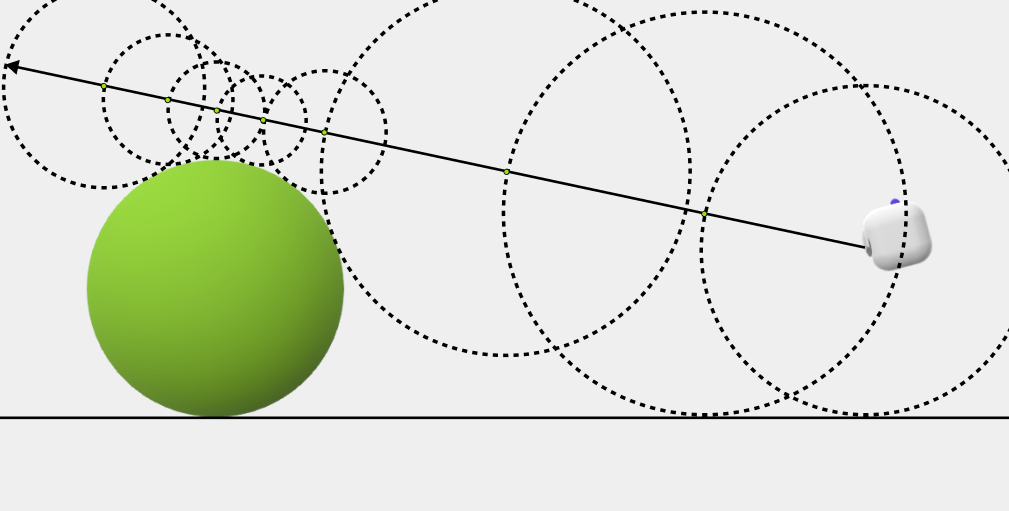
\includegraphics[scale=0.197]{img/C8/sphere-tracing-miss.png} \\
    (a) Encuentra intersección & (b) El rayo se pierde \\[6pt]
    \end{tabular}
    \caption{Posibles estados finales del algoritmo Sphere-Tracing}
    \label{fig:finales}
\end{figure}

\subsection{Signed Distance Functions (SDFs)}
\label{subsection:SDFs}

Como hemos visto, es indispensable para poder aplicar este algoritmo disponer para cada objeto que componga la escena de una función que estime la distancia de un punto cualquiera de $\R^3$ a su superficie. A grandes rasgos, son las conocidas como `Signed Distance Function' (SDFs) las que para una superficie concreta calculan para cualquier punto la distancia estimada a dicha superficie.

Primero explicaremos brevemente el fundamento matemático. Sea $f:\R^n\longrightarrow\R$ una función continua que define implícitamente el conjunto 
$$
A = \{x\in\R^n: f(x)\leq 0\}.
$$
Por continuidad, $f(x)=0\ \ \forall x\in\partial A$. Decimos que la frontera $\partial A$ define la \textit{superficie implícita} de $f$. De hecho, $f$ es negativa en el interior de $A$ ($f(x)<0 \ \ \forall x\in\mathring A$), por lo que podemos decir que dicha superficie implícita $\partial A$ coincide precisamente con el conjunto $f^{-1}(0)$. A partir de una función real y continua podemos entonces definir una superficie en $\R^n$.

\begin{definicion}[SDF]
    Una función continua $f:\R^3\longrightarrow\R$ se conoce como una \textbf{`Signed Distance Bound'} (cota de la distancia con signo) de su superficie implícita $f^{-1}(0)$ si, y solo si
    \begin{equation}
        \label{eq:SDB}
        |f(x)|\leq d(x,f^{-1}(0)) \ \ \forall x\in\R^3
    \end{equation}
    
    Si se tiene la igualdad en (\ref{eq:SDB}), entonces $f$ es una \textbf{`Signed Distance Function'} (función distancia con signo).
\end{definicion}

El caso de las `signed distance bound' también suele ser llamado `BDF' (Bounding Distance Function).

Una forma sencilla de entender este concepto es concibiendo una superficie como los puntos en los que se anula la función distancia. Es decir, si un punto se sitúa a distancia 0 es porque pertenece a dicha superficie. En caso de que la distancia sea positiva en módulo el punto se sitúa fuera, tan lejos como diga dicho módulo.

Como ya hemos visto en la sección anterior, algunas primitivas, como las esferas, pueden ser fácilmente definidas por su SDF. Recordamos de la ecuación (\ref{eq:distancia-punto-esfera}) que la SDF de una esfera es $f(x)=|x-c|-r$ siendo $c\in\R^3$ su centro y $r\in\R$ su radio. Entonces un punto exterior a la esfera tendrá un valor de la SDF positivo, uno interior tendrá un valor negativo y únicamente se anulará en el caso de que el punto pertenezca a la superficie de la esfera (ver imagen \ref{fig:SDF-esfera}).

\begin{figure} [ht]
    \centering
    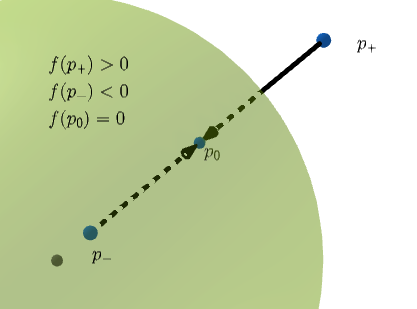
\includegraphics[scale = 0.5]{img/C8/SDF-esfera.png}
    \caption{Ejemplos de puntos con distintos valores de la SDF de una esfera}
    \label{fig:SDF-esfera}
\end{figure}

Otro ejemplo sencillo es el caso de la SDF de un plano. Sea entonces un plano arbitrario $P$ definido por la ecuación $Ax+By+Cz = D$, siendo $\vec N=(A,B,C)$ el vector normal al plano. El punto $p_0$ perteneciente a un plano más cercano a otro punto $p$ dado es aquel que interseca con la recta cuyo vector director es el normal al plano y que pasa por $p$. Es decir, el punto de la recta $S(t)=p+\vec Nt$ que satisface la ecuación $(A,B,C)\cdot (x,y,z) = D$. Veámos para qué $t$ se satisfacen las ecuaciones.
\begin{equation}
    \label{eq:t-mas-cercano}
    \begin{split}
        \vec N\cdot S(t) &= D \\
        \vec N\cdot (p+\vec N t) &= D \\
        t &= \dfrac{D-\vec N \cdot p}{|\vec N|^2}
    \end{split}
\end{equation}
Por tanto la distancia entre punto y plano es la longitud del vector que une a $p$ con $p_0$, véase en la imagen \ref{fig:SDF-plano}.

\begin{figure} [ht]
    \centering
    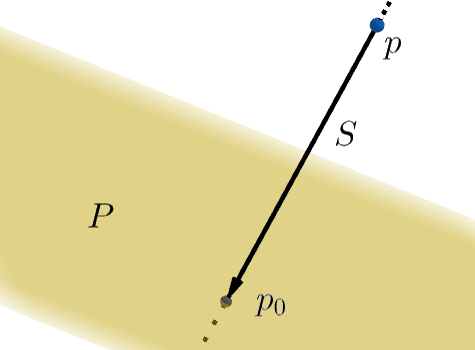
\includegraphics[scale = 0.4]{img/C8/SDF-plano.png}
    \caption{Cálculo de la distancia de un punto a un plano}
    \label{fig:SDF-plano}
\end{figure}

En \cite[Table 1]{Hart-1995} podemos encontrar una lista de primitivas con referencias a sus correspondientes SDFs.

\subsection{Implementación de Sphere-Tracing en pseudocódigo}

Una vez conocemos el funcionamiento intuitivo del algoritmo y la necesidad de SDFs para cada objeto, podemos empezar a pensar en una primera implementación en pseudocódigo del algoritmo. Previamente, necesitamos fijar algunas constantes que sirven como parámetro al algoritmo. Estas constantes son:
\begin{itemize}
    \item $\mathtt{MAX\_STEPS}$: Número máximo de iteraciones o avances en el rayo que se procesarán antes de decidir que el rayo no impacta con ninguna superficie. Es decir, alcanzado dicho número de iteraciones, el algoritmo concluye que el rayo se pierde en el infinito.
    \item \texttt{MAX\_DIST}: Distancia máxima considerada. A distancia del origen del rayo mayor que ésta suponemos que no existe ningún objeto en la escena.
    \item $\varepsilon$: Mínima distancia tal que si en una iteración la distancia mínima calculada es menor que $\varepsilon$ se considera que el punto evaluado pertenece a la superficie del objeto. Claramente un valor pequeño de $\varepsilon$ supone una resolución mayor a cambio de un mayor tiempo de cálculo.
\end{itemize}
Por tanto, el algoritmo, si consideramos un conjunto de $objetos$ (cada uno identificado por un entero $i$, empezando en $0$) y un rayo $R(t)=p_0 + \vec v t$, se describiría como indica el algoritmo \ref{alg:Sphere-Tracing}.

\begin{algorithm}[H]
\caption{Sphere-Tracing} \label{alg:Sphere-Tracing}
\begin{algorithmic}
\Procedure{Sphere-Tracing}{$objects[num\_objects], R(t)= p_0 + \vec v t$}
\State $p\gets p_0$
\State $steps \gets 0$

\While{$steps < \mathtt{MAX\_STEPS}$} \Comment{También se puede fijar una distancia máxima}
    \State $min\_dist \gets \mathtt{MAX\_DIST}$
    \State $i\gets 0$
    
    \While{$i < num\_objects$}\Comment{Cálculo de la mínima distancia de cada iteración}
        \State $dist \gets SDF_{objects[i]}(p)$
        \If{$dist < min\_dist$}
            \State $min\_dist \gets dist$
            \State $index\gets i$
        \EndIf
        \State $i++$
    \EndWhile
    \If{$min\_dist < \varepsilon$}
        \State \textbf{Hay intersección} con $objects[index]$
    \Else
        \State $p\gets p + \vec v \cdot min\_dist$ \Comment{Avanzamos en el rayo}
    \EndIf
    \State $steps++$
\EndWhile

\State \textbf{No existe intersección}
\EndProcedure
\end{algorithmic}
\end{algorithm}

\begin{observacion}
\label{observacion:vector-normalizado}
    Cabe destacar un importante detalle, y es que a partir de este momento es indispensable que en la creación del rayo el vector dirección esté normalizado, pues si queremos avanzar $min\_dist$ unidades en la dirección $\vec v$ y $|v| \not= 1$ se avanzaría una distancia distinta y el algoritmo no funcionaría correctamente, véase imagen \ref{fig:vectores-no-normalizados}.
\end{observacion}

Nótese cómo para el cálculo de la distancia utilizamos funciones distintas que dependen de cada objeto, de ahí el subíndice.

\subsection{Implementación de Shere-Tracing en GLSL}

Veámos ahora cómo podemos llevarnos todos estos nuevos conocimientos a la GPU con GLSL. El objetivo ahora es modificar el fragment shader eliminando la dependencia de \verb|Hit_Sphere| y de \verb|Hit_Plane| para utilizar Sphere-Tracing en el momento de calcular las intersecciones. Realmente el resultado de estas modificaciones debería ser el mismo que en el final del capítulo anterior, pero ahora encontraremos las intersecciones del rayo de forma distinta. 

Lo primero que necesitaremos es una función que calcule la distancia de un punto a una esfera $S$ y otra que calcule la distancia a un plano $P$. Respecto a la esfera, es tan sencillo como implementar una función que calcule la fórmula \ref{eq:distancia-punto-esfera}.

\begin{lstlisting}
// Dada una esfera S y un punto p, calcula la distancia
// del punto a la superficie de la esfera
float get_dist_sphere(vec3 p, Sphere S){
    return length(S.center - p) - S.radius;
}
\end{lstlisting}

Por parte del plano, ya vimos en la sección \ref{subsection:SDFs} cómo calcular la distancia de un punto $p$ a un plano dado por la ecuación $Ax+By+Cz=D$. Primero calculamos el valor de $t$ dado por la ecuación \ref{eq:t-mas-cercano} para así obtener el punto del plano más cercano a $P$, y a partir de ahí obtener la distancia. El código entonces sería:

\begin{lstlisting}
// Dado un plano P y un punto p, calcula la distancia del 
// punto p a la superficie del plano.
float get_dist_plane (vec3 p, Plane P) {
    float t_interseccion = (P.D - dot(P.normal,p))/dot(P.normal, P.normal);
    vec3 closest_point = p + t_interseccion * P.normal;
    return length(p-closest_point);
}
\end{lstlisting}

En realidad podríamos aprovechar que utilizamos como suelo el plano horizontal $y=-2$ y la SDF sería simplemente la componente $y$ del punto $p$ más dos, pero estaríamos limitando la función a este único plano.

Seguidamente necesitamos fijar dos constantes: el número máximo de iteraciones que se darán en el algoritmo (\texttt{MAX\_STEPS}) y $\varepsilon$, la distancia mínima por debajo de la misma se considera que un punto pertenece a la superficie. La primera de ellas la podemos tomar como una macro, al igual que hicimos con el tamaño de los arrays, pero la segunda interesa que sea parametrizable, para así poder observar los niveles de detalle y qué variaciones experimenta la escena al modificar este valor. Por ello, usamos una variable \verb|uniform| a la que pasaremos valor vía JavaScript, que llamaremos \texttt{u\_epsilon}.

\begin{lstlisting}
    uniform float u_epsilon;
    // ... 
    #define MAX_STEPS 1000
\end{lstlisting}

Y ya tenemos todo preparado para implementar el Ray-Marching. La función que dado un rayo calcula posibles intersecciones con los cuerpos y asigna un color es \verb|ray_color|, por lo que lo más natural es editar el código de esta función. En lugar de llamar a \verb|hit_sphere_list| y \verb|hit_plane| como hicimos en la sección \ref{subsection:plano} aplicaremos Ray-Marching. Como GLSL no nos permite mantener un array heterogéneo en el que almacenar todos los objetos independientemente de su tipo, tenemos que hacerlo de forma secuencial. Y como tampoco permite acceder a elementos de un array a partir de índices no constantes, utilizaremos una variable donde almacenar la esfera más cercana, para recuperarla en caso de intersección, véase el código.

\begin{lstlisting}
vec4 ray_color(Ray r, Sphere S[ARRAY_TAM], int num_spheres, 
    Plane ground,
    Directional_light lights[ARRAY_TAM], int num_lights) {
    
    Hit_record hr; hr.hit = false;  // Hit_record structure
    float dist = MAX_DIST;          // Distancia a cada objeto 
    vec3 p = r.orig;                // Punto del rayo
    float closest_dist = MAX_DIST;  // Menor distancia
    float current_t = 0.0;          // p=orig+current_t*dir
    vec4 tmp_color;                 // Color temporal
    Sphere S_hit;                   // Esfera mas cercana
    
    int object_index;   // 0,...,num_spheres-1: esferas,
                        // num_spherees: plano
    // Ray Marching
    for(int i = 0; i < MAX_STEPS; i++) {
        // Calculamos el objeto mas cercano
        closest_dist = MAX_DIST;

        // Distancia a las esferas
        for(int i = 0; i < ARRAY_TAM; i++) {
            if(i == num_spheres) break;
            dist = get_dist_sphere(p, S[i]);
            if(dist < closest_dist) {
                closest_dist = dist;
                object_index = i;
                S_hit = S[i];
            }
        }

        // Distancia al suelo
        dist = get_dist_plane(p, ground);
        if(dist < closest_dist) {
            closest_dist = dist;
            object_index = num_spheres;
        }
    
        // closest_dist almacena la menor de las distancias
        // y object_index el indice del objeto mas cercano
        if(closest_dist < u_epsilon){   // Hay interseccion

            hr.hit = true;
            hr.t = current_t;
            hr.p = ray_at(r, hr.t);

            if(object_index == num_spheres){ // Suelo
                // Codigo de interseccion con el suelo ...
            }

            else {      // Una de las esferas
                // Codigo de interseccion con S_hit
            }
        }

        // Si no hay interseccion, avanzamos en el rayo
        current_t += closest_dist;
        p = ray_at(r, current_t);

        // Si estamos muy lejos acabamos el bucle
        if(current_t >= MAX_DIST) break;
    }
    // No hay interseccion
    // Background code ...       
}
\end{lstlisting}

Fíjese que concuerda con la estructura que describe el algoritmo \ref{alg:Sphere-Tracing}. Hecha esta modificación, el resultado fijando ciertos parámetros dinámicamente es el mostrado en la imagen \ref{fig:esferas-ST}. Tal y como adelantamos, el resultado es igual que cuando calculábamos las intersecciones exactas, ya que realmente lo único que cambia es la forma de calcular las intersecciones, nada estrictamente visual.

\begin{figure} [ht]
    \centering
    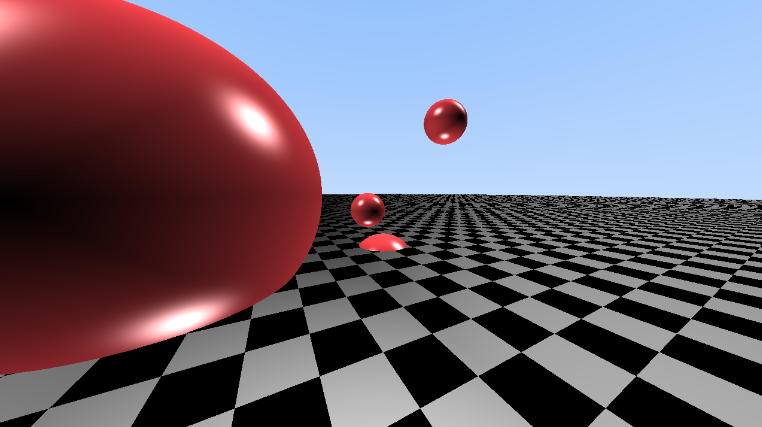
\includegraphics[scale = 0.37]{img/C8/esferas-ray-marching.png}
    \caption{Escena tras implementar Sphere Tracing}
    \label{fig:esferas-ST}
\end{figure}

Recordamos e insistimos en que el vector director del rayo \verb|r.dir| debe ser un vector normalizado, es decir, unitario. De otro modo los avances en el rayo no estarán controlados, obsérvese en la imagen \ref{fig:vectores-no-normalizados} los resultados obtenidos al no normalizar el vector director al crear el rayo.

\begin{figure} [ht]
    \centering
    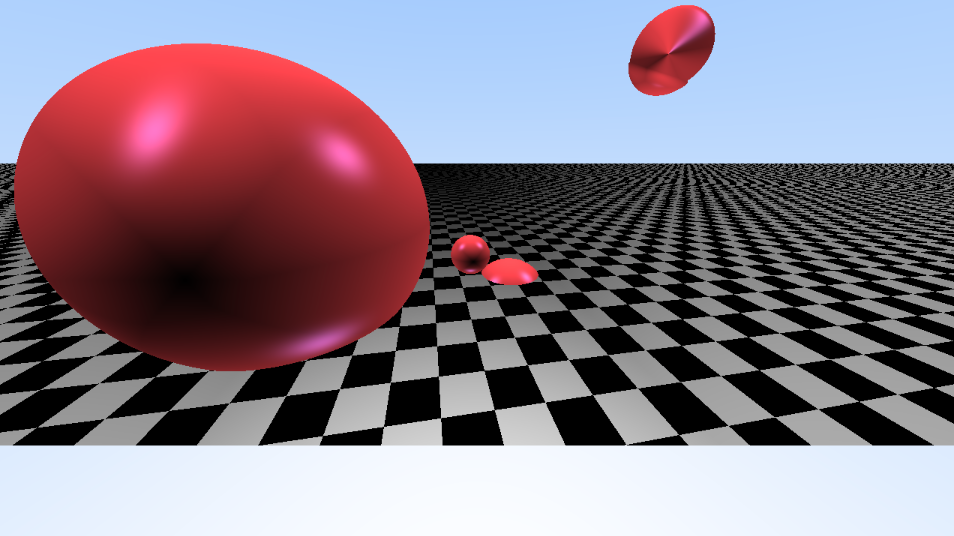
\includegraphics[scale = 0.3]{img/C8/vectores-no-normalizados.png}
    \caption{Escena utilizando vectores no unitarios en los rayos}
    \label{fig:vectores-no-normalizados}
\end{figure}

\subsection{Comentarios sobre Sphere-Tracing}
\label{subsection:comentarios}

Una vez hemos introducido e implementado el algoritmo Sphere-Tracing, el lector es posible que piense que es una forma menos exacta y además menos eficiente que calcular analíticamente las intersecciones con los cuerpos. Es cierto que en casos como el de esferas o planos, cuyas ecuaciones implícitas y sus intersecciones con rayos están muy bien definidos y son sencillas de calcular, aplicar sphere-tracing ralentiza el procesado. Sin embargo, muchas superficies, como es el caso de los fractales, no cuentan con una ecuación implícita que la defina. Otras sí cuentan con ecuaciones implícitas pero estas son muy difíciles de resolver. En este último caso se pueden aplicar métodos numéricos para aproximar las soluciones, que son métodos precisamente iterativos. 

Sin embargo, sphere-tracing sólo necesita, para cada cuerpo, una función que aproxime suficientemente bien la distancia a un conjunto, o al menos una cota inferior, y esta cota disminuya conforme el rayo se acerca al conjunto. Sería suficiente una cota inferior porque esta nos aseguraría que al avanzar en el rayo no nos pasamos de largo al avanzar en el rayo. Lo único que debemos garantizar es que la cota inferior debe tener exactamente los mismos ceros que la original (es decir, nunca es cero donde la original no lo es). De hecho, se puede usar esto en casos donde la función distancia exacta sea muy difícil o imposible de calcular.

En concreto, podemos usar cualquier función $f$ que tenga exactamente los mismos ceros que la función distancia exacta y que sea lipschitziana, es decir, que existe una constante positiva $K$ tal que

$$
|f(p)-f(q)|\leq K \|p-q\| \ \ \forall p,q\in\R^3 
$$
de tal forma que si llamamos $p_0$ al punto de la superficie más cercano a $p$, por hipótesis $f(p_0)=0$, por lo que

$$
|f(p)|\leq K \| p-p_0\|
$$

Si tomamos la función $g=f/K$, directamente se tendría 

$$
|g(p)|\leq\|p-p_0\|
$$
Convirtiendo a $g$ en una cota inferior de la distancia a $p_0$ (una BDF), por lo que podemos utilizar a $g$ para aplicar sphere tracing.

Sin embargo, si tomamos una cota inferior en lugar de la exacta, al dar pasos más pequeños, se tiene menos eficiencia. Dicho esto, queda claro que la función distancia exacta de un punto a la superficie es la mejor opción, pues es lipschitziana por definición y su constante es de Lipschtiz es $1$, pero por dificultad en su cálculo se suelen usar cotas inferiores.

Por tanto, a partir de un rayo y dichas funciones se puede aplicar sphere-tracing, de forma que se converge finalmente al punto de intersección. Por contra, si buscamos intersecciones analíticas hay que resolver ecuaciones, en ocasiones para acabar aproximando las soluciones, y retener la más pequeña. 

Un aspecto a destacar de sphere-tracing es la dependencia de sus parámetros. Es importante fijar un valor $\varepsilon$ adecuado, ya que si es demasiado grande puede brindarnos resultados muy pobres. En la imagen \ref{fig:esferas-ST} se ha utilizado $\varepsilon=0.001$ y nos da un resultado muy bueno, pero obsérvese en la imagen \ref{fig:epsilon-grande} qué ocurre si se fija $\varepsilon=0.1$. Los límites de los cuadrados del suelo se distorsionan y las apariencias de las esferas también se ven muy resentidas. No obstante, es cierto que a mayor valor de $\varepsilon$ menos iteraciones y por tanto más velocidad, pero los resultados son peores. Es por tanto necesario utilizar valores de $\varepsilon$ adecuados a la situación, siendo suficientemente pequeños como para obtener un buen resultado pero suficientemente grandes como para que sea computacionalmente viable.

\begin{figure} [ht]
    \centering
    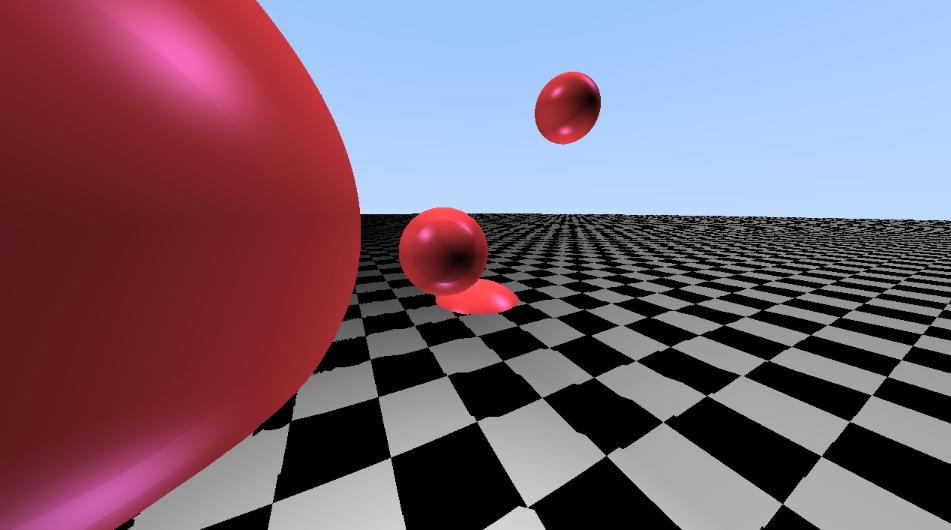
\includegraphics[scale = 0.3]{img/C8/epsilon-grande.png}
    \caption{Escena generada utilizando $\varepsilon=0.1$}
    \label{fig:epsilon-grande}
\end{figure}

Una reflexión similar se puede aplicar al parámetro que define el número máximo de iteraciones (\verb|MAX_STEPS|). Pensemos en un rayo que pasa muy cerca de un objeto pero no llega a intersecarlo, sino que finalmente interseca al suelo. Durante las iteraciones que el rayo pase cerca del objeto quizá avance muy lentamente durante varias iteraciones, pues la distancia mínima es la distancia a dicho objeto que es pequeña. Este hecho puede provocar que se alcance el número máximo de iteraciones, considerando así que el rayo no golpea ningún objeto y asignándole el color de fondo cuando realmente con algunas iteraciones más podría alcanzarse la intersección con el suelo. Este hecho se puede observar en la imagen \ref{fig:pocas-iteraciones}, donde se ha utilizado \verb|MAX_STEPS=100|. Fíjese en las fronteras entre el horizonte y las esferas, o en los bordes de las esferas.

\begin{figure} [ht]
    \centering
    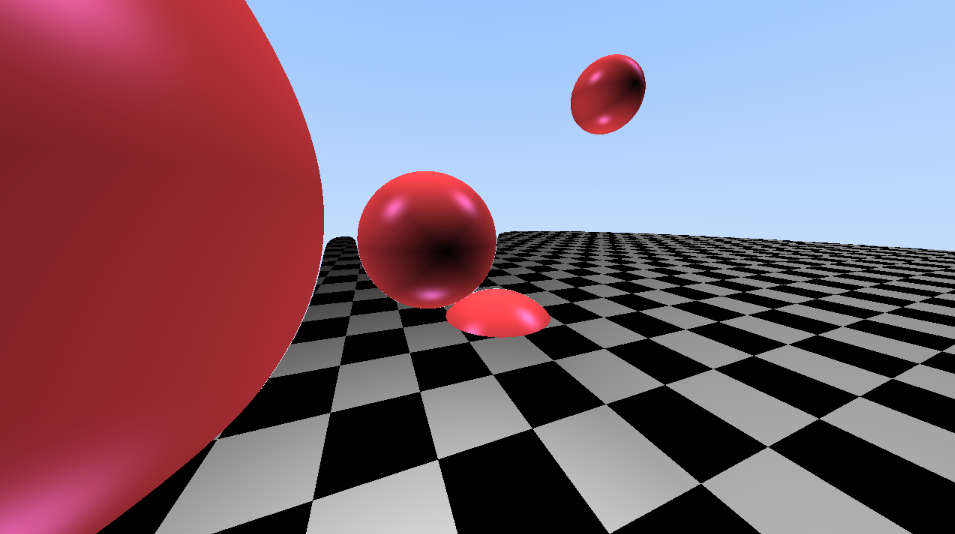
\includegraphics[scale = 0.3]{img/C8/pocas-iteraciones.png}
    \caption{Escena generada utilizando $\mathtt{MAX\_STEPS}$=100}
    \label{fig:pocas-iteraciones}
\end{figure}

De igual forma, menos iteraciones implica más rapidez, pero peores resultados, por lo que es necesario fijar un valor correcto.

\section{Visualización tridimensional de conjuntos de Julia}

Una vez tenemos definido el algoritmo que usaremos para la visualización de fractales, que es el algortimo de ray-marching acompañado de una SDF concreta, es momento de trabajar en la visualización de fractales 3D. Comenzaremos, siguiendo el mismo orden que adoptamos en el capítulo \ref{chap:fractales-2D}, por los conjuntos de Julia en 3D.

Recordemos de la sección \ref{section:Julia} que el conjunto de Julia $\mathcal{J}_c$ de un número complejo fijo $c\in\C$ se define como la frontera entre el conjunto de puntos prisioneros y el conjunto de puntos de escape bajo la iteración de la función $P_{c}(z)=z^2+c$. Es decir, $\mathcal{J}_c = \partial \mathsf{E}_c$, donde
\begin{equation}
    \mathsf{E}_c = \{z_0\in\C: \{|P_c^n(z_0)|\}\rightarrow \infty \}
\end{equation}

Queda por tanto a la vista una clara dependencia de los números complejos en esta definición, los cuales podemos identificar únicamente con puntos del plano euclídeo $\R^2$. Necesitamos por tanto una generalización tridimensional de los números complejos. Estrictamente, no existe como tal una generalización tridimensional que mantenga la aritmética compleja, pero sí que existe una en cuatro dimensiones: los cuaternios, usualmente denotados como $\H$.

Podemos encontrar información sobre los cuaternios en \cite{quaternions}, pero introduciremos brevemente su aritmética. De igual forma que para los números complejos se utiliza la unidad imaginaria $i$, en los cuaternios se tienen tres unidades imaginarias: $i,j,k$, de tal manera que un cuaternio se compone de una parte real y tres imaginarias, pudiendo expresarlo como:
\begin{equation}
    q = a i + b j + c k + d \cong (a,b,c,d)\in \R^4.
\end{equation}

Nótese que estamos denotando como componente real a $w$, la última de la terna $(x,y,z,w)$. Las unidades imaginarias se multiplican entre ellas siguiendo las siguien reglas:
\begin{equation}
    \label{eq:relaciones-cuaternios}
    \begin{split}
        ij = k \quad jk &= i \quad ki = j \\
        ji = -k \quad kj &= -i \quad ik = -j \\
        i^2 = j^2 &= k^2 = -1. 
    \end{split}
\end{equation}

Lo cual nos da a entender que los cuaternios tienen estructura de anillo no conmutativo. Una forma de calcular el producto de dos cuaternios arbitrarios $q = q_x i + q_y j + q_z k + q_w\cong (q_x,q_y,q_z,q_w)$ y $q' = q'_x i + q'_y j + q'_z  k + q'_w\cong (q'_x,q'_y,q'_z,q'_w)$ es expandiendo la expresión

\begin{equation}
    qq' = (q_x i + q_y j + q_z k + q_w)(q'_x i + q'_y j + q'_z k + q'_w) 
\end{equation}

Si utilizamos su expresión como ternas de $\R^4$, denotando $q=(q_{xyz},q_w), q'=(q'_{xyz},q_w)$, agrupando términos y aplicando las relaciones \ref{eq:relaciones-cuaternios} el resultado puede expresarse mediante productos vectoriales y escalares:
\begin{equation}
    \label{eq:producto-cuaternios}
    \begin{split}
        (qq')_{xyz} &= q_{xyz}\times q'_{xyz} + q_w q'_{xyz} + q'_wq_{xyz} \\
        (qq)_w &= q_wq'_w - (q_{xyz}\cdot q'_{xyz})
    \end{split}
\end{equation}

Aplicando estas relaciones podemos deducir el cuadrado de un cuaternio con tan solo multiplicarlo por sí mismo, obteniendo

\begin{equation}
    \label{eq:cuadrado-cuaternio}
    \begin{split}
        (q^2)_{xyz} &= 2q_w q_{xyz} \\
        (q^2)_w &= q_w^2 - q_{xyz}\cdot q_{xyz},
    \end{split}
\end{equation}
que realmente es una simplificación de las ecuaciones (\ref{eq:producto-cuaternios}) teniendo en cuenta que el producto vectorial de un vector por sí mismo es $0$.

Y una vez tenemos clara la aritmética básica de los cuaternios, podemos generalizar fácilmente los conjuntos de Julia sin más que extender la función $P_c(z)$ a $\H$, fijando un cuaternio $c\in\H$:
\begin{equation}
    \label{eq:f-julia-cuaternios}
    \begin{split}
        P_c :& \H \longrightarrow \H \\
        q & \longmapsto q^2 + c
    \end{split}
\end{equation}

De forma que ahora separamos el espacio $\H$ en puntos prisioneros y de escape frente a la iteración de $P_c(q)$ y redefinimos los conjuntos de Julia en 4D como la frontera entre los puntos prisioneros y de escape. 

Sin embargo, es claro que no podemos visualizar conjuntos en 4D de forma tan directa como lo hacemos en 2D, pero sí podemos generarlos y visualizar una proyección en 3D. Pensemos en los mapas de curvas de nivel que se usan en topografía (imagen \ref{fig:curva-de-nivel}), los cuales fijando una altura concreta representan la curva que dibujaría una montaña al intersecarla con un plano horizontal situado a esa altura, permitiéndonos hacernos una idea de la forma en 3D de la montaña a partir de un plano en 2D. 

\begin{figure} [ht]
    \centering
    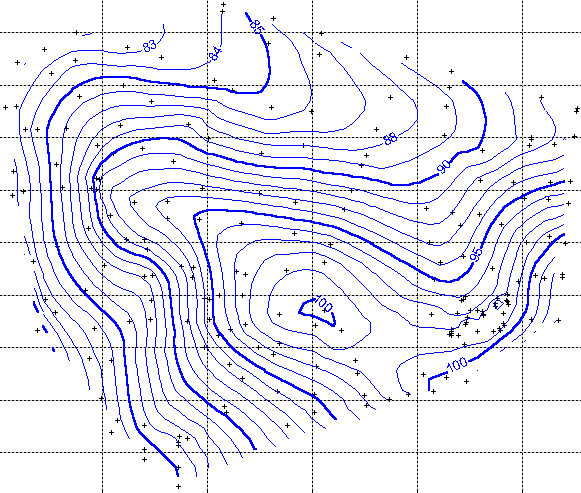
\includegraphics[scale = 0.3]{img/C8/curvas-de-nivel2.png}
    \caption{Representación de una montaña con curvas de nivel}
    \label{fig:curva-de-nivel}
\end{figure}

En nuestro contexto, podemos fijar una dimensión y visualizar el conjunto de Julia para las otras tres. 

Es por tanto momento de estimar la distancia de un punto cualquiera $p\in\R^3$ a un conjunto de Julia $\mathcal{J}_c$, con $c\in\H$. Lo primero es indentificar un punto del espacio euclídeo $(x,y,z)\in\R^3$ con un cuaternio. La forma que escogeremos será identificando $x$ con la parte real y la segunda y tercera componente con las dos primeras componentes imaginarias, fijando a $0$ la tercera componente imaginaria ($k$). Es decir,
\begin{equation}
    p=(x,y,z)\cong q = x + yi + zj \cong (y,z,0,x)
\end{equation}

Es posible que parezca antinatural identificar $(x,y,z)$ con $(y,z,0,x)$, pero si utilizamos la relación $(x,y,z)\cong xi+yj+zk$ anulando la parte imaginaria, los conjuntos de Julia que se calculen serían todos esferas concéntricas, lo cual carece de interés \cite{Hart-1989}.

Tengamos en cuenta que en principio los rayos van a partir de un punto que está fuera del conjunto de Julia, es decir, al iterar la función $P_c$ la sucesión va a ser divergente, por lo que la SDF nos debe de dar una distancia positiva. La idea es que cada vez nos dé un valor menor conforme nos acerquemos a $\mathcal{J}_c$ hasta prácticamente anularse en caso de que el rayo interseque con el conjunto. 

Debemos por tanto antes de nada iterar $q$ para hacernos a la idea de esta distancia al conjunto, de forma que si tras cierto número $M$ de iteraciones el módulo de la iterada $|P_c^M(q)|$ no es suficientemente grande consideraremos que el punto es convergente, aunque esto probablemente ocurra únicamente si se evalúa en un punto muy cercano a la superficie del conjunto. Es decir, iteramos el punto con una amplia posibilidad de que antes o después la $n$-ésima iterada tenga un módulo grande, y en caso contrario la iterada convergerá a algún valor tras las $M$ iteraciones. Denotamos como $q_n=P_c^n(q)$ a esta $n$-ésima iterada. A partir de este cuaternio, definimos la SDF del conjunto de Julia como 
\begin{equation}
    \label{eq:SDF-Julia}
    \begin{split}
        d_c&:\R^3\longrightarrow\R \\
        d_c(p) &= \dfrac{|q_n|\log|q_n|}{2|q'_n|}
    \end{split}
\end{equation}

donde $q'_n$ es otra sucesión iterativa que se puede calcular conjuntamente con $q_n$ mediante $q'_{i+1}=2q_i q'_i$, comenzando con $q'_0=1\cong(0,0,0,1)$, aunque como realmente sólo necesitamos su módulo podemos calcular $|q'_{i+1}|=2|q_i||q'_i|$\footnote{El módulo de un cuaternio es $|xi+yj+zk+w|=\sqrt{x^2+y^2+z^2+w^2}$}. Esta sucesión $q'_n$ es la derivada de $q_i$ respecto de $q_0$, calculada iterativamente según la regla de la cadena, es decir
\begin{equation}
    \begin{split}
        q'_{i+1}&=\frac{\partial P^{i+1}_c(q_0)}{\partial q_0}\\
        &= \frac{\partial}{\partial q_0}\left((P_c^i(q_0))^2+c\right)\\
        &= 2 P_c^i(q_0)(P_c^i)'(q_0)\\
        &= 2 q_i q'_i
    \end{split}
\end{equation}

La función \ref{eq:SDF-Julia} es una aproximación de la distancia real, concretamente una cota inferior, la cual se basa en el potencial de Hubbard-Douady, tal y como se describe en \cite{Hubbard-Douady}[Capítulo 8]. Para ello se usa la posibilidad de usar BDFs que se mencionó en el apartado \ref{subsection:comentarios}.

Sabemos hasta ahora que iterando el punto inicial y aplicando la transformación (\ref{eq:SDF-Julia}) podemos estimar a qué distancia se sitúa el punto del conjunto de Julia $\mathcal{J}_c$. 

\subsection{Aproximando la normal}
\label{subsection:normal-sdf}

Teniendo esta estimación de la distancia podemos calcular el posible punto de intersección de un rayo con $\mathcal{J}_c$, pero si queremos evaluar el modelo de iluminación en dicho punto, antes necesitamos conocer la normal a la superficie en dicho punto. Y aquí es donde tenemos que afrontar la dificultad que supone la propia belleza de los fractales, que es su irregularidad y que su superficie en general no es diferenciable. Por ello, no existe un plano tangente a la superficie ni un vector normal a la misma en ninguno de sus puntos. Sin embargo, nosotros estamos aproximando esa superficie ideal con otra distinta, muy similar, pero no igual, y esa otra superficie aproximada sí es diferenciable, por lo que podemos utilizar ciertos métodos para aproximar esta normal.

\subsubsection{Método 1: Gradiente de la SDF}

La manera más sencilla de obtener un vector normal a la superficie es tomando el gradiente de la SDF, el cual evidentemente no calculamos analítica sino numéricamente utilizando diferencias centradas. Para ello, fijado un punto $p\in\R^3$, calculamos 6 puntos muy próximos a él, sumando y restando en cada una de sus tres componentes un pequeño incremento, que por simplicidad consideraremos que será el propio $\varepsilon$ que fijamos al hacer ray-marching. En cada uno de los 6 puntos evaluamos la SDF y calculamos para cada componente la diferencia, tomando como normal el vector formado por cada una de estas diferencias divididas normalizado.

\begin{algorithm}[H]
    \caption{Cálculo de la normal mediante el gradiente de la SDF} \label{alg:normal-gradiente-sdf}
    \begin{algorithmic}
    \Procedure{CalcularNormalGradiente}{$p$: punto de $\R^3$, $d_c$: SDF del objecto}
        \State $h\gets\varepsilon$
        \State $g_{x+}\gets p + (h,0,0)$
        \State $g_{x-}\gets p - (h,0,0)$
        \State $g_{y+}\gets p + (0,h,0)$
        \State $g_{y-}\gets p - (0,h,0)$
        \State $g_{z+}\gets p + (0,0,h)$
        \State $g_{z-}\gets p - (0,0,h)$

        \State $\nabla d_{c_x} \gets d_c(g_{x+})-d_c(g_{x-})$
        \State $\nabla d_{c_y} \gets d_c(g_{y+})-d_c(g_{y-})$
        \State $\nabla d_{c_z} \gets d_c(g_{z+})-d_c(g_{z-})$
            \State \textbf{return} $\dfrac{(\nabla d_{c_x},\nabla d_{c_y},\nabla d_{c_z})}{\|(\nabla d_{c_x},\nabla d_{c_y},\nabla d_{c_z})\|}$
    \EndProcedure
    \end{algorithmic}
\end{algorithm}

En realidad debería tomarse en cada componente del gradiente la diferencia dividida entre $2h$, pero la propia normalización del vector se encarga de reescalar el vector adecuadamente.    

\subsubsection{Método 2: Técnica del tetraedro}

Consideramos un tetraedro cuyos vértices son $k_0=(1,-1,-1)$, $k_1=(-1,-1,1)$, $k_2=(-1,1,-1)$ y $k_3=(1,1,1)$. Sean ahora los puntos $p_i := p+\varepsilon k_i\ \ i=0,\dots,3$. Entonces una aproximación de la normal a la superficie en el punto $p$ es la normalización del vector $\sum_{i=0}^3 k_i d_c(p_i)$. Consúltese \cite{normals-sdf} si se desea tener una justificación del funcionamiento de este método.

\begin{algorithm}[H]
    \caption{Técnica del tetraedro para el cálculo de normales} \label{alg:normal-tetraedro}
    \begin{algorithmic}
    \Procedure{CalcularNormalTetraedro}{$p$: punto de $\R^3$, $d_c$: SDF del objecto}
    \State $h\gets\varepsilon$
    \State $p_0 \gets p + h(1,-1,-1)$
    \State $p_1 \gets p + h(-1,-1,1)$
    \State $p_2 \gets p + h(-1,1,-1)$
    \State $p_3 \gets p + h(1,1,1)$

    \State $N\gets \sum_{i=0}^3 k_i d_c(p_i)$

    \State \textbf{return} $\dfrac{N}{\|N\|}$
    \EndProcedure
    \end{algorithmic}
\end{algorithm}

\subsection{Implementación en GLSL}

Tenemos por tanto ya la forma de calcular tanto la distancia de un punto al conjunto de Julia de un $c\in\H$ fijo como un método para calcular la normal a la superficie del fractal en un punto, dos de hecho. Es por tanto momento de la implementación. Basta con programar funciones que calculen la SDF y sustituir las llamadas a \verb|get_dist_sphere| por una llamada a dicha función, y una vez se conoce el punto de intersección calcular la normal y evaluar el modelo de iluminación.

De manera natural, igual que identificamos un cuaternio con un elemento de $\R^4$ utilizaremos el tipo \verb|vec4| para representar a los mismos en GLSL. Recordemos que en este caso es la última componente la parte real del cuaternio.

\begin{lstlisting}
vec4 q; // Representa un cuaternio (a,b,c,d)
// q = ai + bj + cz + d
\end{lstlisting}

Si ahora seguimos la ecuación (\ref{eq:cuadrado-cuaternio}) podemos rápidamente implementar una función que dado un cuaternio calcule su cuadrado.

\begin{lstlisting}
// Dado un cuaternio q, calcula su cuadrado q^2
vec4 quat_square(vec4 q){
    vec3 xyz = 2.0*q.w*q.xyz;
    float w = q.w*q.w - dot(q.xyz, q.xyz);
    return vec4(xyz, w);
}
\end{lstlisting}

Por lo que gracias a esta función y a la aritmética ya programada es sencillo programar la función $P_c(q)=q^2+c$. Utilizamos una función para iterar el cuaternio asociado a un punto $p$, aprovechando la posibilidad que nos ofrece GLSL de simular el paso de parámetros por referencia mediante las variables \verb|out| e \verb|inout|. En el último caso, una función recibe un parámetro y en caso de que su valor cambie durante la ejecución éste mantiene su valor tras el retorno de la función. El código es 
\begin{lstlisting}
// Itera la funcion P_c y obtiene tanto q_n como |q'_n|
// q: Cuaternio que se itera
// dq: Sucesion |q'_n|
// c: Constante fija de P_c asociada al conjunto de Julia
void iterate_julia(inout vec4 q, inout float dq, vec4 c) {
    for(int i = 0; i < 50; i++) {   // 50 son suficientes
        dq = 2.0 * length(q) * dq;
        q = quat_square(q) + c;     // P_c(q) = q^2 +c
        if(dot(q, q) > 64.0) break;    // |q| es grande
    }
}
\end{lstlisting}

Fíjese que esta función itera un cuaternio mediante la función $P_c(q)$ y a la vez calcula la sucesión recurrente $|q'_{i+1}|=2|q_n||q'_n|$. 

Por tanto, el cálculo de la distancia de un punto $p$ al conjunto $\mathcal{J}_c$ se reduce a identificar $p\in\R^3$ con un cuaternio $q\in\H$, iterar $q$ y $|q'|$ teniendo en cuenta que la iteración de $q'$ comienza en $1$ y aplicar la función (\ref{eq:SDF-Julia}).

\begin{lstlisting}
float get_dist_julia(vec3 p, vec4 c) { 
    vec4 q = vec4(p.y, p.z, 0.0, p.x);
    float dq = 1.0;     // q'_0 = 1
    iterate_julia(q, dq, c);
    float length_q = length(q);
    return 0.5*length_q * log(length_q) / dq;
}
\end{lstlisting}

Y ya tenemos implementada la SDF de Julia. únicamente resta un método para calcular normales. Como hemos presentado dos, implementaremos los dos, utilizando ahora compilación condicional mediante macros para decidir cuál emplear. Tan solo tenemos que implementar los algoritmos \ref{alg:normal-gradiente-sdf} y \ref{alg:normal-tetraedro}. % TODO Seguimos con esto?

\begin{lstlisting}
#define NORMAL 0 // O 1
// Calcula la normal al conjunto J_c en el punto p
vec3 calculate_normal_julia(vec3 p, vec4 c) {
    vec3 N;
    float h = u_epsilon;

    #if NORMAL == 0
    // Gradiente de la SDF
    vec4 qp = vec4(p.y, p.z, 0.0, p.x);
    float gradX, gradY, gradZ;
    vec3 gx1 = (qp - vec4( 0.0, 0.0, 0.0, h )).wxy;
    vec3 gx2 = (qp + vec4( 0.0, 0.0, 0.0, h )).wxy;
    vec3 gy1 = (qp - vec4( h, 0.0, 0.0, 0.0 )).wxy;
    vec3 gy2 = (qp + vec4( h, 0.0, 0.0, 0.0 )).wxy;
    vec3 gz1 = (qp - vec4( 0.0, h, 0.0, 0.0 )).wxy;
    vec3 gz2 = (qp + vec4( 0.0, h, 0.0, 0.0 )).wxy;
    
    gradX = (get_dist_julia(gx2,c) - get_dist_julia(gx1,c))/(2.0*h);
    gradY = (get_dist_julia(gy2,c) - get_dist_julia(gy1,c))/(2.0*h);
    gradZ = (get_dist_julia(gz2,c) - get_dist_julia(gz1,c))/(2.0*h);
    N = normalize(vec3( gradX, gradY, gradZ ));

    #else
    // Metodo del tetraedro
    const vec2 k = vec2(1,-1);
    N = normalize( k.xyy*get_dist_julia( p + k.xyy*h, c ) + 
                   k.yyx*get_dist_julia( p + k.yyx*h, c ) + 
                   k.yxy*get_dist_julia( p + k.yxy*h, c ) + 
                   k.xxx*get_dist_julia( p + k.xxx*h, c ) );

    #endif
    return N;
}
\end{lstlisting}

Y ya únicamente resta sustituir en el ray-marching las SDFs y el método para calcular normales de las esferas por el código que corresponde a los conjuntos de Julia. Para poder dinamizar el cuaternio $c\in\H$ que se considera fijo en los cálculos declaramos una variable \verb|uniform| al igual que se hizo a la hora de los conjuntos de Julia 2D. También creamos una variable global que es \verb|Material fractal_material;| que como su propio nombre indica es el material que se le asignará al objeto fractal.

\begin{lstlisting}
// Cuaternio c fijo. Visualizaremos el conjunto J_c
uniform vec4 u_juliaSetConstant;
// Material que se asigna al fractal
Material fractal_material
// ...

vec4 ray_color(Ray r, Plane ground, 
    Directional_light lights[ARRAY_TAM], int num_lights) {

    // ... 
    int object_index; // 0: Ground, 1: Julia

    // Ray Marching
    for(int i = 0; i < MAX_STEPS; i++) {
        closest_dist = MAX_DIST;
        // Distancia al plano
        dist = get_dist_plane(p, ground);
        if(dist < closest_dist) {
            closest_dist = dist;
            object_index = 0;
        }
        // Distancia a Julia
        dist = get_dist_julia(p , u_juliaSetConstant);
        if(dist < closest_dist){
            closest_dist = dist;
            object_index = 1;
        }

        if(closest_dist < u_epsilon){   // Hay interseccion
            hr.hit = true;
            hr.t = current_t;
            hr.p = ray_at(r, hr.t);
            if(object_index == 0){      // r hits the ground
                // ... 
            else {      // r hits Julia
                hr.mat = fractal_material;
                hr.normal = calculate_normal_julia(
                    hr.p, u_juliaSetConstant);
            return evaluate_lighting_model(lights, num_lights, hr);
        }
        current_t += closest_dist;
        p = ray_at(r, current_t);
        if(current_t >= MAX_DIST) break;
    }
    // r does not hit nothing
    // ... 
}
\end{lstlisting}

Y con esta modificación de \verb|ray_color| podemos ya visualizar conjuntos de Julia tridimensionales. Podemos también cambiar los parámetros del material para observar distintas apariencias. 

En las imágenes \ref{fig:julia-3D} podemos ver algunos de los resultados que, después de este largo camino, hemos podido obtener modificando los parámetros.

\begin{figure}[ht]
    \centering
    \begin{tabular}{cc}
      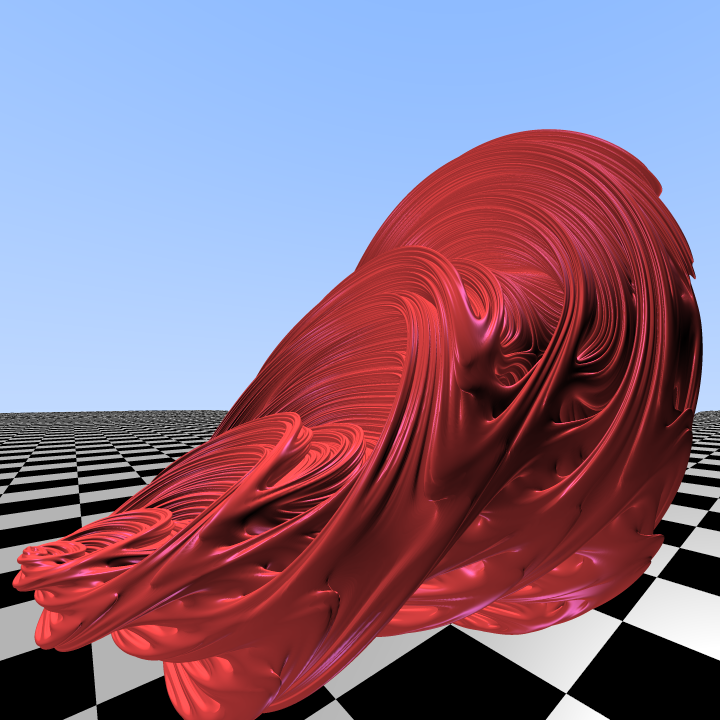
\includegraphics[scale=0.28]{img/C8/julia-1.png} &     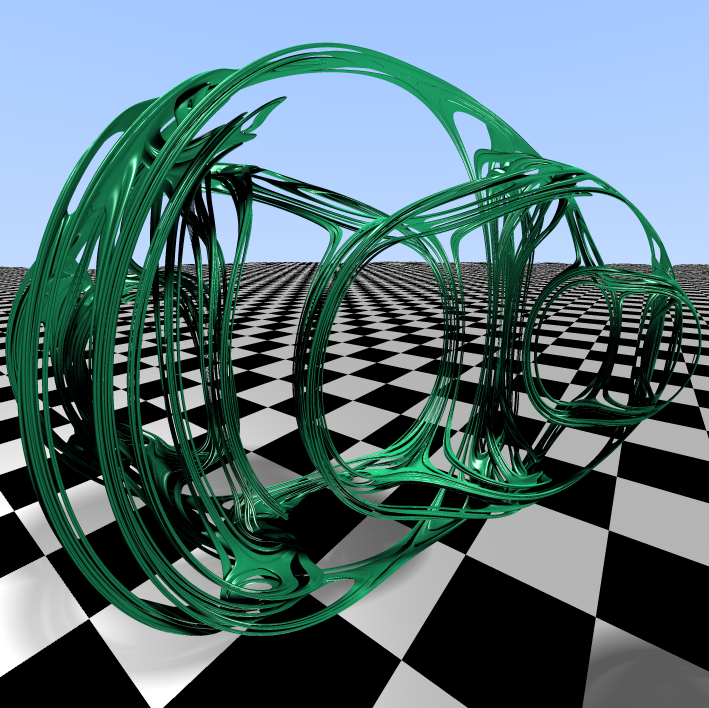
\includegraphics[scale=0.36]{img/C8/julia-2.png} \\
    (a) $c=-0.12+0.75 i$ & (b) $c=0.3+1.09j+0.3k$ \\[6pt]
    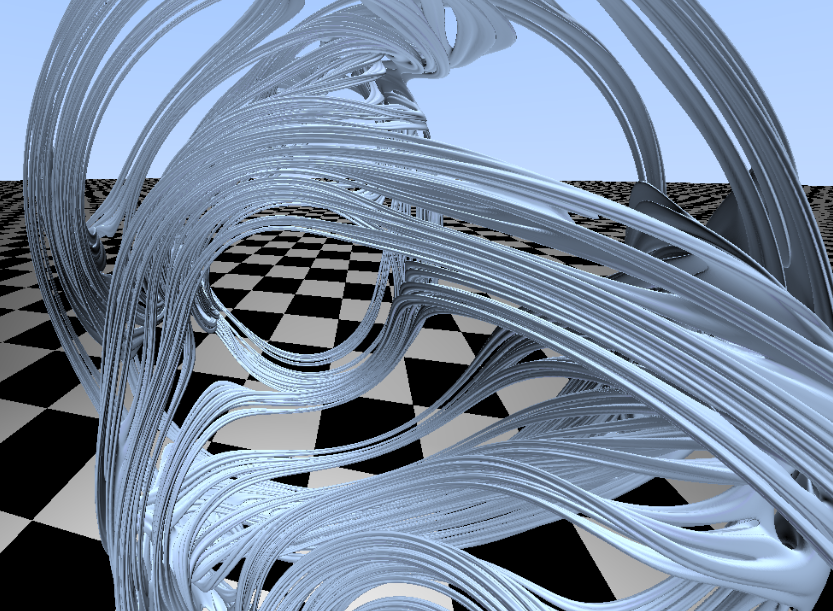
\includegraphics[scale=0.21]{img/C8/julia-3.png} &     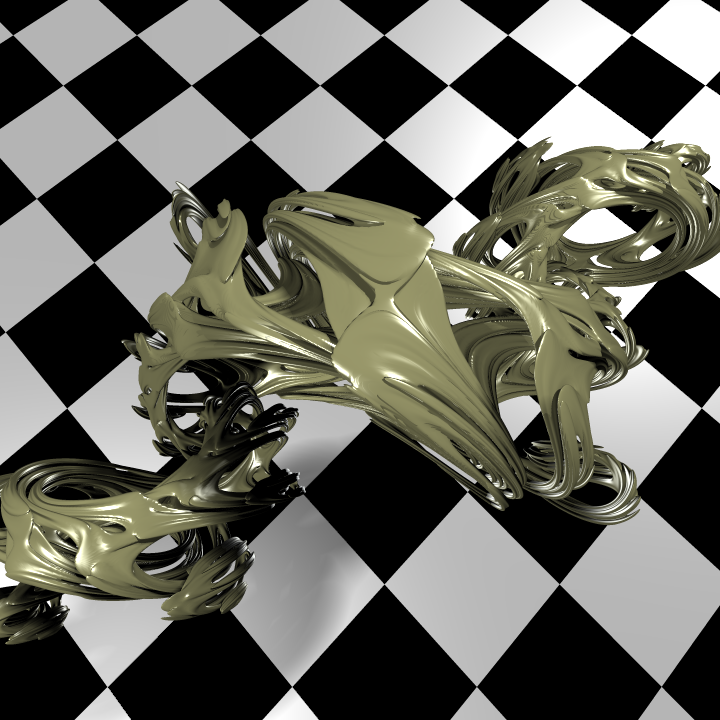
\includegraphics[scale=0.25]{img/C8/julia-4.png} \\
    (c) $c=0.1+0.74i+0.62j+0.14k$ & (d) $c=-0.81-0.48j-0.1k$ \\[6pt]
    \end{tabular}
    \caption{Conjuntos de Julia 3D para distintos $c\in\H$}
    \label{fig:julia-3D}
\end{figure}

\section{Visualización tridimensional del conjunto de Mandelbrot}
\label{section:Mandelbrot-3D}

La pregunta más natural tras visualizar conjuntos de Julia es si podemos aprovechar todo el código que tenemos para, bajo ligeras modificaciones, visualizar lo que sería el conjunto de Mandelbrot en 3D. Afortunadamente, la respuesta es sí. Recordemos ahora la sección \ref{section:Mandelbrot}, en la cual definimos, en $\C$, al conjunto de Mandelbrot $\mathcal{M}$ de varias formas equivalentes, entre las que destacamos
$$
\mathcal{M}=\{c\in\C : \{P_c^n(0)\}\not\rightarrow\infty\}
$$

Por tanto, la manera de iterar $q$ y $q'$ cambia levemente. En lugar de utilizar un cuaternio $q_0$ como semilla e iterar $q^2+c$ con un $c\in\H$ fijo, utilizaremos a $0$ como semilla e iteraremos $q^2+c$ con $c=q_0$. La iteración de $|q'|$ también cambia, ya que intuitivamente la derivada de la función que iteramos es $2qq'+1$, por lo que ahora la sucesión sería $|q'_{i+1}|=2|q_i||q'_i|+1$, con $q'_0=0$. Puede consultarse una explicación más detallada de esta diferencia en \cite{distance-fractals}.Finalmente, tras suficientes iteraciones, se obtienen los valores $q_n$ y $q'_n$ necesarios en la SDF.

\begin{lstlisting}
// Itera la funcion P_c y obtiene tanto q_n como |q'_n|
// q: Cuaternio que se itera
// dq: Sucesion |q'_n|
void iterate_mandelbrot(inout vec4 q, inout float dq) {
    vec4 c = q;     // Constante inicialmente igual a q
    q = vec4(0.0);  // Semilla inicial
    for(int i = 0; i < 50; i++) {
        dq = 2.0 * length(q) * dq + 1.0;
        q = quat_square(q) + c;
        if(dot(q, q) > 64.0) break;
    }
}
\end{lstlisting}

Salvo esta diferencia, la función que calcula la distancia de un punto al conjunto de Mandelbrot generalizado es idéntica a la utilizada en conjuntos de Julia: 
$$
d(p)=\dfrac{|q_n|\log|q_n|}{2|q'_n|},
$$
teniendo en cuenta las diferencias existentes entre estos $q_n$ y $q'_n$ con respecto a los utilizados en Julia.

\begin{lstlisting}
float get_dist_mandelbrot(vec3 p) {
    float dist;
    vec4 q = vec4(p.y, p.z, 0.0, p.x);
    float dq = 0.0;
    iterate_mandelbrot(q, dq);
    float length_q = length(q);
    return 0.5*length_q * log(length_q) / dq;
}
\end{lstlisting}

Por su parte, los métodos para aproximar la normal descritos en la sección \ref{subsection:normal-sdf} son igualmente válidos no sólo para este caso sino realmente para cualquier superficie, ya que son considerados métodos estándar de cálculo de normales. Por tanto podemos reutilizarlos sin más que cambiar las llamadas a \verb|get_dist_julia| por llamadas a \verb|get_dist_mandelbrot|. 

Y una vez tenemos estas funciones, podemos modificar \verb|ray_color| para que en lugar de utilizar las funciones de Julia utilice las de Mandelbrot. Sin embargo, en lugar de cambiar la actual, añadiremos funcionalidad. De igual manera que en la sección \ref{subsection:alternando} explicamos que añadiendo una variable \verb|uniform| la cual en función de su valor se graficará un conjunto u otro, en este caso haremos exactamente lo mismo, añadir una variable \verb|uniform| llamada \verb|u_fractal| y en función de su valor invocaremos la SDF y el método para calcular normales de Julia o de Mandelbrot.

\begin{lstlisting}
uniform int u_fractal; // 1: Julia, 2: Mandelbrot 
\end{lstlisting}

Tras esta pequeña modificación y darle a \verb|u_fractal| el valor $2$ mediante JavaScript, mostramos el resultado de estas operaciones en las imágenes \ref{fig:mandelbrot-3D}.

\begin{figure}[ht]
    \centering
    \begin{tabular}{cc}
        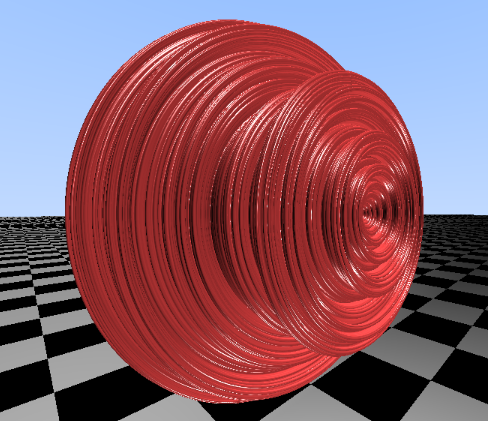
\includegraphics[scale=0.33]{img/C8/mandelbrot-2.png} &
      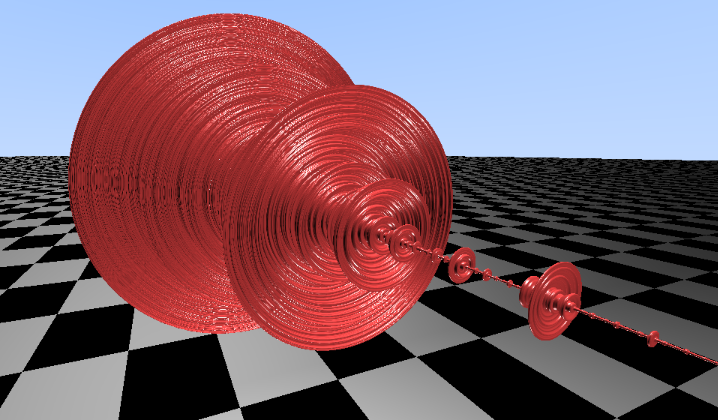
\includegraphics[scale=0.33]{img/C8/mandelbrot-1.png} \\    
    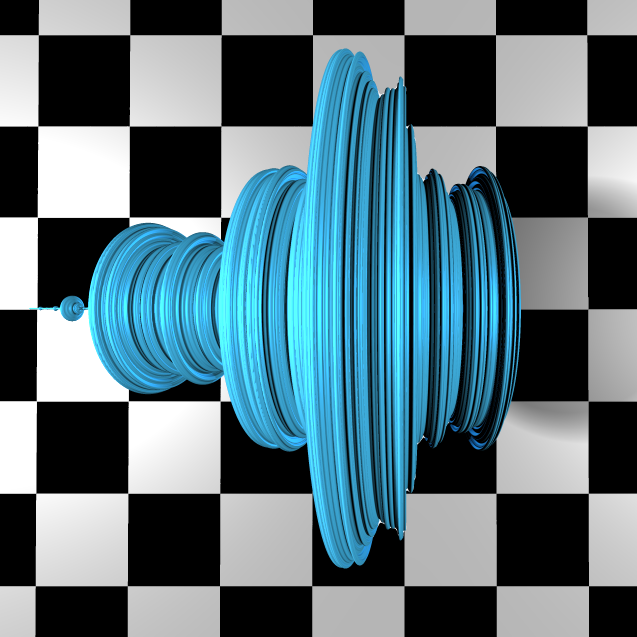
\includegraphics[scale=0.4]{img/C8/mandelbrot-3.png} &     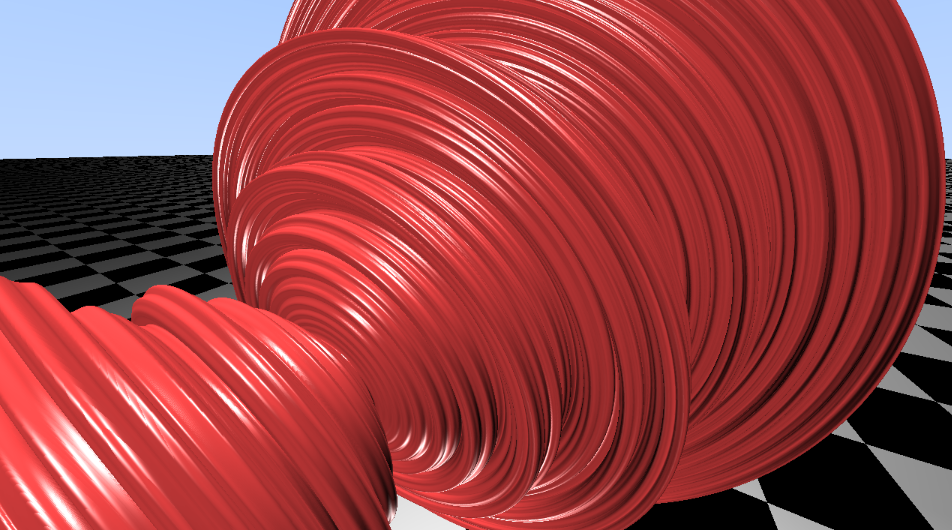
\includegraphics[scale=0.25]{img/C8/mandelbrot-4.png} \\
    \end{tabular}
    \caption{Detalles del conjunto de Mandelbrot generalizado}
    \label{fig:mandelbrot-3D}
\end{figure}

Hay que reconocer que el resultado es un poco decepcionante, parecería un cuerpo generado por la revolución de la frontera del conjunto de Mandelbrot 2-dimensional en torno al eje $X$.

\section{El conjunto de Mandelbub}

Gracias a los cuaternios hemos podido generalizar la definición de los números complejos a 4D y visualizar en 3D proyecciones de los conjuntos de Julia y el conjunto de Mandelbrot. Sin embargo, la apariencia del conjunto de Mandelbrot nos ha dejado un mal sabor de boca, y es que dista bastante de la belleza que nos ofrecía $\mathcal{M}$ en dos dimensiones. En realidad, a día de hoy no se ha conseguido ninguna generalización matemáticamente correcta que posea la complejidad y la belleza del conjunto de Mandelbrot en 2D, aunque ha habido varios intentos. El conjunto de Mandelbub es uno de estos intentos. Es una generalización tridimensional del conjunto de Mandelbrot alejada del álbegra que ofrecen cuaternios, hipercomplejos y otros tipos de álgebras, a veces inconsistentes. 

Pensemos en $P_c(z)=z^2+c$, esta vez con $z,c\in\C$ como la operación que, dado un complejo $z$ multiplica su módulo por sí mismo, duplica su argumento y suma una cierta constante $c$. Si recurrimos en 3D a las coordenadas esféricas, las cuales identifican un punto $p\in\R^3$ mediante su módulo $r$, el ángulo que forma con el plano $y=0$ ($\phi$) y el ángulo que forma con el eje X ($\theta$), podemos extender esta operación. El procedimiento sería pasar el punto $p=(x,y,z)$ de coordenadas cartesianas a esféricas $(r,\phi,\theta)$, elevar al cuadrado $r$, duplicar $\phi$ y $\theta$ y devolver a coordenadas cartesianas. Es decir, tendríamos la composición 

$$
(x,y,z)\longmapsto(r,\phi,\theta)\longmapsto(r^2,2\phi,2\theta)\longmapsto(x',y',z')
$$

Realmente, el álgebra, las operaciones, las `derivadas' utilizadas en este procedimiento y en el cálculo de la distancia al objeto no tiene ningún rigor ni fundamento matemático, pero el resultado que produce es mucho más satisfactorio.

De igual manera que utilizamos el $2$ como exponente, podemos usar cualquier otro. En este contexto lo más usual es usar el 8, ya que para exponentes más altos se tiende a la simetría y a detalles menos marcados. De manera que la transformación que usaremos entonces es la función $f$ que actúa sobre $p=(x,y,z)$ de la siguiente forma

\begin{equation}
    \label{eq:f-Mandelbub}
    f(p)=f(x,y,z) = \Phi(|p|^8,8\phi, 8\theta),
\end{equation}
donde $\Phi$ es la función que pasa de coordenadas esféricas a cartesianas, es decir
$$
\Phi(r,\phi,\theta) = (r\sin(\phi)\sin(\theta),r\cos(\phi),r\sin(\phi)\cos(\theta))
$$
y donde $\phi = \arccos(\frac{y}{|p|})$ y $\theta=\arctan(\frac{x}{z})$.

El procedimiento, en lo que se refiere a iterar un punto para posteriormente estimar la distancia al objeto es bien parecido al ya conocido, solo que en este caso en lugar de utilizar la potencia y suma de cuaternios utilizamos la transformación (\ref{eq:f-Mandelbub}). Y claro está a la hora de calcular lo que entonces conocíamos como $q'$ la iteración cambia al haber cambiado el exponente. En este caso sería $|w'_{i+1}|=8|w|^7|w'|+1$, de forma que, dado un punto $w\in\R^3$, debemos calcular las iteraciones 
\begin{align*}
    w_{i+1} &= f(w_i), & w_0&=w \\
    |w'_{i+1}| &= 8|w_i|^7|w'_i|+1, & w'_0&=1
\end{align*}
Tomando para $f$ como $c$ el valor de $w$ inicial.

Una vez $w$ y $|w'|$ han sido suficientemente iteradas, tenemos el punto $w_n$ y el módulo $|w'_n|$, dispuestos a aplicarle la SDF que de nuevo es la transformación \ref{eq:SDF-Julia}. Consúltese \cite{mandelbub} para más información sobre la SDF.

Como dijimos anteriormente, el método del gradiente de la SDF y el método del tetraedro descritos en la sección \ref{subsection:normal-sdf} son igualmente válidos para cualquier superficie supuesta conocida su SDF. Por lo que podemos también calcular las normales al conjunto de Mandelbub a partir de estos métodos.

La implementación necesaria para la visualización del conjunto de Mandelbub se basa en programar la función $f$ (la transformación \ref{eq:f-Mandelbub}), una función que itere un punto concreto y la sucesión de `derivadas', una que invoque a la iteración y calcule la estimación de la distancia y otra que calcule las normales.

Respecto de la primera, podemos aprovechar que la GPU es muy rápida calculando funciones trigonométricas. Existen alternativas polinómicas que evitan el uso de trigonometría, la cual suele ser lenta en CPU, pero como en GPU suelen ser más rápidas, haremos uso de estas. 
\begin{lstlisting}
vec3 f_Mandelbub(vec3 w, vec3 c) {
    // Coordenadas esfericas
    float wr = sqrt(dot(w,w));
    float wo = acos(w.y/wr);
    float wi = atan(w.x,w.z);
    // Escalado y rotacion
    wr = pow( wr, 8.0 );
    wo = wo * 8.0;
    wi = wi * 8.0;
    // Vuelta a coordenadas cartesianas
    w.x = wr * sin(wo)*sin(wi);
    w.y = wr * cos(wo);
    w.z = wr * sin(wo)*cos(wi);
    return c + w;
}
\end{lstlisting}

Seguidamente, una función que invoque a \verb|f_Mandelbub| para iterar \verb|w| y \verb|dw|. Puede llamar la atención que en este caso se rompa el bucle cuando la longitud supera el valor 2 en contraste con los 8 que se utilizan en los conjuntos de Julia y Mandelbrot, pero se ha comprobado empíricamente que de esta forma los resultados son óptimos. Además 10 iteraciones a lo sumo son también suficientes, ya que elevar el módulo a $8$ es una transformación que en general cambia muchísimo los valores por lo que la convergencia o divergencia es rápida.

\begin{lstlisting}
// Itera un punto de R^3 segun la funcion f_Mandelbub y
// calcula tambien la sucesion de derivadas
void iterate_mandelbub(inout vec3 w, inout float dw){
    float m;
    vec3 c = w;
    for(int i = 0; i < 10; i++) {
        m = length(w);      // |z|
        dw = 8.0*m*m*m*m*m*m*m*dw + 1.0; // 8*|z|^7*z' + 1.0
        w = f_Mandelbub(w,c);   // w_n^8 + w_0
        if(m > 2.0) break;     // |z| > 2
    }
}
\end{lstlisting}

Por último, la función que definitivamente dado un punto $p\in\R^3$ devuelve la distancia al conjunto de Mandelbub. 

\begin{lstlisting}
float get_dist_mandelbub(vec3 p) {
    vec3 w = p;
    float dw = 1.0;
    iterate_mandelbub(w,dw);    // Iteramos w y dw
    float length_w = length(w);        // |w|
    return 0.5*length_w * log(length_w) / dw;
}
\end{lstlisting}

Con este nuevo código junto con el necesario para calcular las normales y las modificaciones necesarias para que se represente el conjunto de Mandelbub según el valor de \verb|u_fractal|, ya podemos visualizar el mismo. 

\begin{figure}[ht]
    \centering
    \begin{tabular}{cc}
        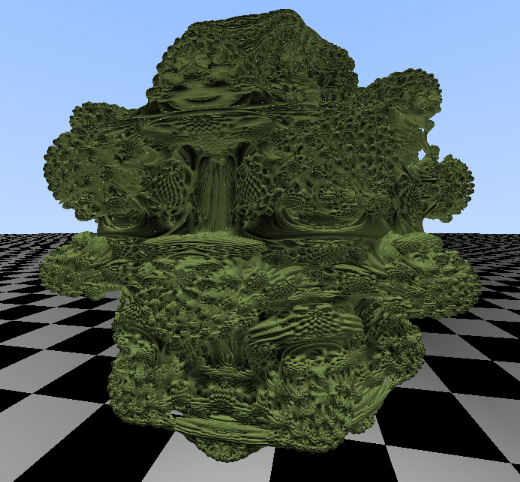
\includegraphics[scale=0.34]{img/C8/mandelbub-1.png} &
      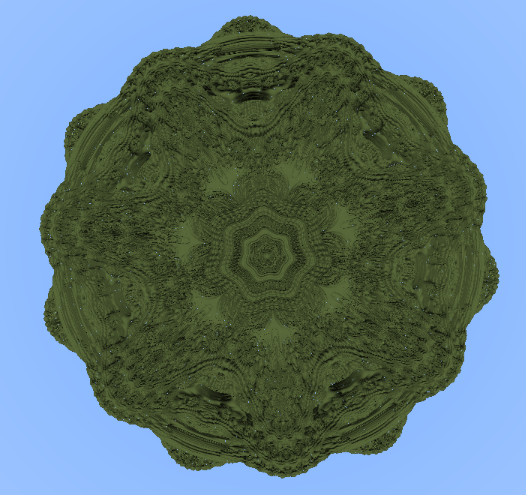
\includegraphics[scale=0.33]{img/C8/mandelbub-2.png} \\    
    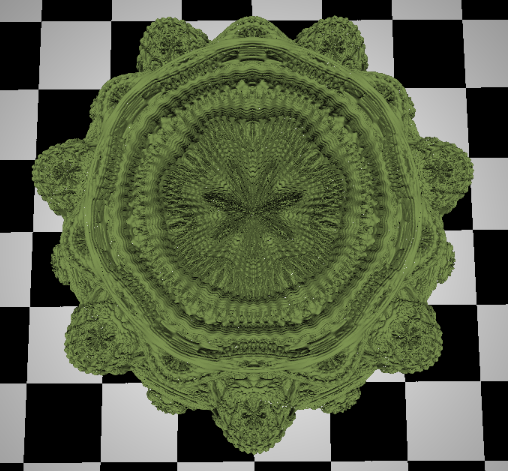
\includegraphics[scale=0.35]{img/C8/mandelbub-3.png} &     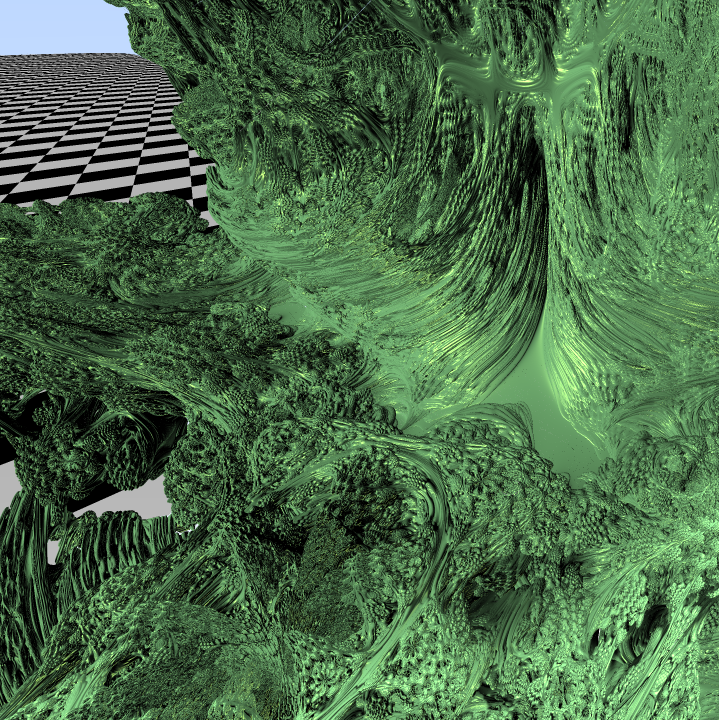
\includegraphics[scale=0.31]{img/C8/mandelbub-4.png} \\
    \end{tabular}
    \caption{Conjunto de Mandelbub}
    \label{fig:mandelbub}
\end{figure}

Nótese como efectivamente mejora por mucho el resultado que nos ofrecía el conjunto de Mandelbrot generalizado a cuaternios de las imágenes \ref{fig:mandelbrot-3D}. Sin embargo, recordamos que el álgebra y el rigor utilizado para visualizarlo está lejos de ser correcto, siendo aún así el resultado más llamativo hasta ahora. Este es el colofón a toda la teoría y todas las implementaciones que se han hecho desde que se inició con un cuadrado de colores en el capítulo \ref{chap:visualizacion}, pudiendo al fin observar fractales tridimensionales desde distintas perspectivas, con distintos materiales y por tanto diferentes apariencias.


\section{Comparación con los fractales 2D}

En las secciones anteriores y a lo largo de todo el recorrido que hemos hecho desde el capítulo \ref{chap:visualizacion}, el objetivo era conseguir generalizar a tres dimensiones los fractales del capítulo \ref{chap:Julia-Mandelbrot} y que con ayuda de WebGL pudimos revisualizar en el \ref{chap:fractales-2D}: conjuntos de Julia y Mandelbrot. Es por tanto momento de comparar los resultados obtenidos en 2D con los resultados obtenidos en 3D.

\subsection{Comparación entre conjuntos de Julia 2D y 3D}

Los conjuntos de Julia generalizados a tres dimensiones no son sino proyecciones a partir de un punto $p=(x,y,z)\in\R^3$ identificándolo con un cuaternio al cual se le anula su última componente imaginaria $q=x + yi +zj + 0k\in\H$. En particular, podemos tomar la tercera componente también como nula e identificar un punto $p'=(x,y)\in\R^2$ con un cuaternio $q'=x + yi + 0j + 0k\in\H$, y como además $i^2=-1$, podemos restringir la aritmética de los cuaternios a la de los complejos. Esto, a nivel teórico, nos lleva a decir que si tomamos los puntos del plano $z=0$, los identificamos con un cuaternio y los iteramos bajo $P_c(q)=q^2+c$ el resultado es precisamente el conjunto de Julia 2-dimensional.

Es decir, la sección provocada por el plano $z=0$ en los conjuntos de Julia 3D debe coincidir con los conjuntos de Julia 2D (no olvidemos que el conjunto en sí es la frontera entre conjuntos prisioneros y de escape). Esto se puede apreciar bastante bien si observamos el conjunto $\mathcal{J}_{-1}$ en 3D, que a la vista queda su parecido con su análodo 2-dimensional, fíjese en la figura \ref{fig:julia-3D-2D}.

\begin{figure}[ht]
    \centering
    \begin{tabular}{cc}
        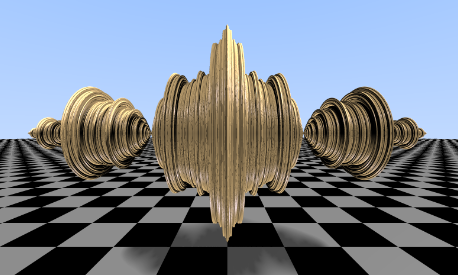
\includegraphics[scale=0.37]{img/C8/julia-3D-frontal-1.png} &
      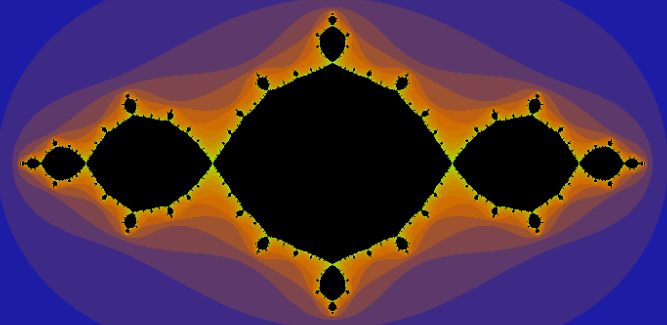
\includegraphics[scale=0.31]{img/C8/julia-2D-1.png} \\    
    (a) En 3D & (b) En 2D  \\
    \end{tabular}
    \caption{Conjunto $\mathcal{J}_{-1}$}
    \label{fig:julia-3D-2D}
\end{figure}

De hecho, la generalización tridimensional es la superficie generada por la revolución del conjunto en 2D en torno al eje $X$, fíjese en la vista ofrecida por la figura \ref{fig:julia-3D-abajo-1}. Esto de hecho ocurre con todos los conjuntos de Julia de números puramente reales (se puede comprobar interactuando con la web \url{https://jantoniovr.github.io/Geometria-Fractal/3D-fractals.html}).

\begin{figure} [ht]
    \centering
    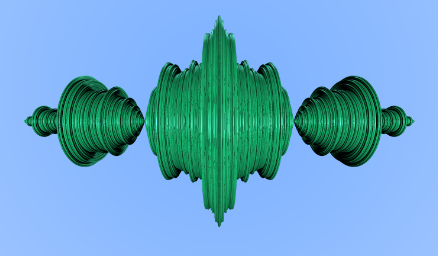
\includegraphics[scale = 0.5]{img/C8/julia-3D-abajo-1.png}
    \caption{$\mathcal{J}_{-1}$ visto desde abajo}
    \label{fig:julia-3D-abajo-1}
\end{figure}

De igual manera que anulando la componente en $z$ se obtiene en la sección del plano $z=0$ el conjunto 2D, si se anula la componente en $y$ y se libera la $z$ pasa lo propio en el plano $y=0$. Fíjese como la sección de $\mathcal{J}_{-0.71-0.31i}$ en el plano $z=0$ (imagen \ref{fig:julia-3D-varias} (a)) es la misma que la de $\mathcal{J}_{-0.71-0.31j}$ en el plano $y=0$ (imagen \ref{fig:julia-3D-varias} (b)).

\begin{figure}[ht]
    \centering
    \begin{tabular}{cc}
        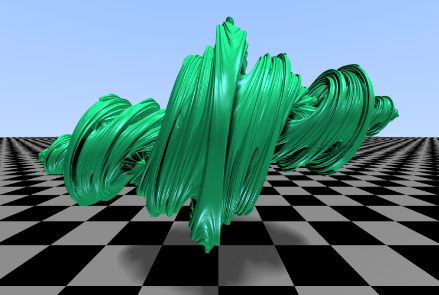
\includegraphics[scale=0.4]{img/C8/julia-3D-frontal-2.png} &
      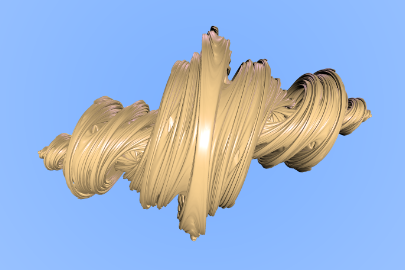
\includegraphics[scale=0.44]{img/C8/julia-3D-abajo-2.png} \\    
    (a) $\mathcal{J}_{-0.71-0.31i}\subseteq\H$ & (b) $\mathcal{J}_{-0.71-0.31j}\subseteq\H$  \\
    \end{tabular}
    \caption{Generalizaciones de $\mathcal{J}_{-0.71-0.31i}\subseteq\C$}
    \label{fig:julia-3D-varias}
\end{figure}

Además, aunque los detalles 3D no nos dejan apreciar claramente las similitudes entre el conjunto $\mathcal{J}_{-0.71-0.31i}$ en $\C$ y en $\H$, en la figura \ref{fig:julia-2D-3D-2} podemos observar ciertos parecidos entre los bulbos que tiene el fractal en 3D a su derecha y los que tiene el fractal en 2D.

\begin{figure}[ht]
    \centering
    \begin{tabular}{cc}
        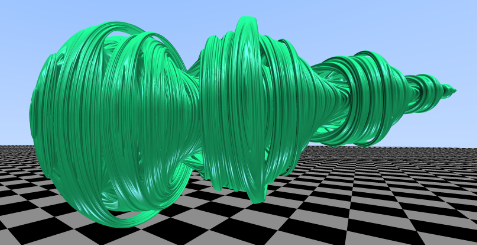
\includegraphics[scale=0.42]{img/C8/julia-3D-oblicuo-2.png} &
        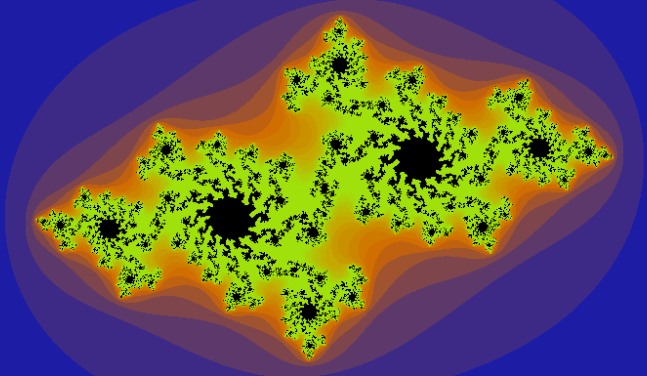
\includegraphics[scale=0.28]{img/C8/julia-2D-2.png} \\
          
    (a) Detalle en 3D & (b) En 2D  \\
    \end{tabular}
    \caption{Conjunto $\mathcal{J}_{-0.71-0.31i}$}
    \label{fig:julia-2D-3D-2}
\end{figure}

\subsection{Comparación entre el conjunto de Mandelbrot 2D y 3D}

De manera análoga a lo explicado para conjuntos de Julia basados en la iteración de cuaternios, un cuaternio $q=x+yi+0j+0k$ puede ser identificado con un número complejo $x+yi$. Entonces, si un complejo $c=c_x+c_yi\in\C$ pertenece a $\mathcal{M}$, necesariamente un cuaternio $q=c_x+c_yi+0j+0k$, el cual en 3D se identifica con un punto $(c_x,c_y,0)$ perteneciente al plano $z=0$, debe también pertenecer al conjunto de Mandelbrot en 3D. Entonces, el conjunto de Mandelbrot tridimensional debe dibujar al conjunto de Mandelbrot 2D en el plano $z=0$. Análogamente, esto también ocurre en el plano $y=0$ si anulamos la coordenada en $y$ en lugar de la $z$. Nos remitimos a la sección \ref{section:Mandelbrot-3D} y a las imágenes \ref{fig:mandelbrot-3D} para recordar que la generalización 3D no era más que la superficie generada por la revolución de $\mathcal{M}$ en torno al eje $X$, por lo que queda comprobada la propiedad que acabamos de describir.

No obstante, en las imágenes \ref{fig:mandelbrot-2D-3D} presentamos algunas imágenes comparativas para que se pueda apreciar directamente la similitud entre $\mathcal{M}$ en 2D y en 3D. Precisamente por la revolución dejan de observarse a simple vista detalles como los bulbos o la cardioide que constituye el cuerpo principal de $\mathcal{M}$.

\begin{figure}[ht]
    \centering
    \begin{tabular}{cc}
        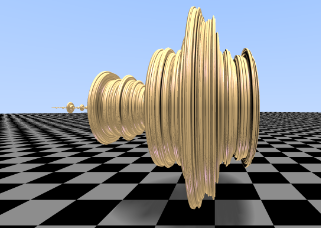
\includegraphics[scale=0.53]{img/C8/mandelbrot-3d.png} &
        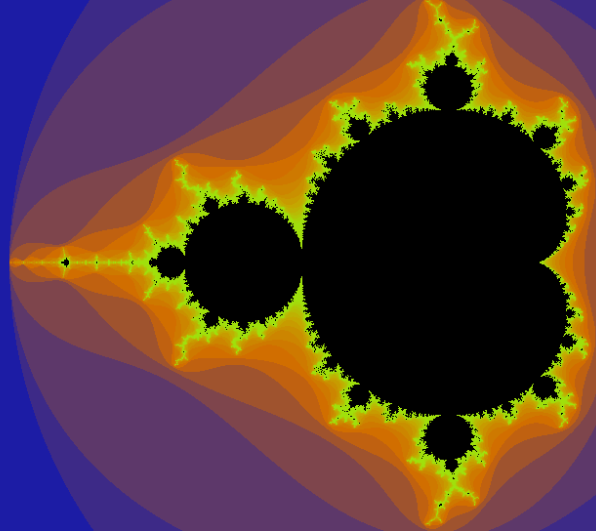
\includegraphics[scale=0.23]{img/C8/mandelbrot-2d.png} \\
          
    (a) En 3D & (b) En 2D  \\
    \end{tabular}
    \caption{Conjunto de Mandelbrot}
    \label{fig:mandelbrot-2D-3D}
\end{figure}

\subsection{Comparación entre el conjunto de Mandelbub y $\mathcal{M}_8$}

En realidad el conjunto de Mandelbub no es sino una forma de generalizar, de forma matemáticamente poco precisa, el conjunto de Mandelbrot de orden 8, el cual nos remitimos a la sección \ref{subsection:julia-mandelbrot-generalizados} para recordar su génesis. En la imagen \ref{fig:mandelbubbrot} (b) podemos recordar el aspecto que tenía $\mathcal{M}_8$. Aparentemente, está dividido en lo que parecen 7 regiones, cada una con infinitos bulbos donde destaca uno que es más grande que los demás. 

La parte de Mandelbub que más recuerda a $\mathcal{M}_8$ es la parte inferior (imagen \ref{fig:mandelbubbrot} (a)), que aunque no es igual, también se aprecia que está dividida en 7 regiones iguales. A su vez, el propio cuerpo de Mandelbub tiene 7 salientes en cada uno de sus dos niveles (imagen \ref{fig:mandelbub}), haciendo cierta analogía con $\mathcal{M}_8$. 

\newpage

\begin{figure}[ht]
    \centering
    \begin{tabular}{cc}
        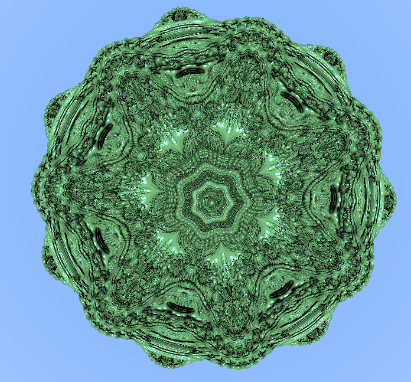
\includegraphics[scale=0.46]{img/C8/mandelbub-abajo.png} &
        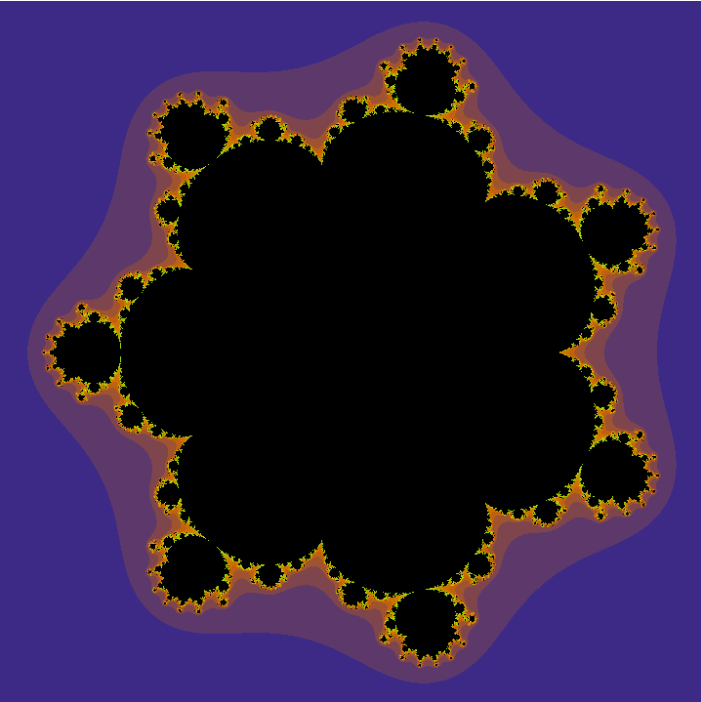
\includegraphics[scale=0.25]{img/C8/M-8.png} \\
          
    (a) Vista desde abajo de Mandelbub & (b) $\mathcal{M}_8$  \\
    \end{tabular}
    \caption{Conjunto de Mandelbub y de Mandelbrot de orden 8}
    \label{fig:mandelbubbrot}
\end{figure}



\section{Efectos realistas en la escena}

Una vez hemos conseguido visualizar objetos de naturaleza fractal en una escena 3D, debemos cuidar el realismo y las apariencias de la escena. Esto lo conseguiremos modificando el modelo de iluminación para que el fractal proyecte sombras arrojadas en el suelo y sobre sí mismo y mediante la técnica conocida como antiliasing.

\subsection{Sombras arrojadas}
\label{subsection:sombras}

En la sección \ref{section:Phong} dotamos a nuestra escena de un modelo de iluminación y de dos fuentes de luz que alumbran los objetos que componen la escena, pero no nos preocupamos de la posible sombra que causen estas fuentes de luz en el plano que consideramos como suelo o las sombras que pueda provocar un fractal sobre sí mismo. Es momento por tanto de graficar estas posibles sombras.

En las ecuaciones del modelo de Phong tuvimos en cuenta que si la luz no incide sobre el punto, no se calcularían posibles efectos de iluminación difusa y especular. Esto se hizo pensando que si el coseno del ángulo que forman la dirección de la luz y la normal al objeto en el punto es cuestión es positivo entonces la fuente incide sobre el punto, en caso contrario la fuente de luz no alcanza el punto (imagen \ref{fig:excepcion}). Sin embargo, si lo pensamos, esta condición es suficiente únicamente en objetos convexos, ya que no pueden estar en la sombra de sí mismos en ningún caso. Pensemos por ejemplo en el tubo de la imagen \ref{fig:objeto-no-convexo}. Aunque el coseno de $\theta$ sea positivo, el punto señalado quedaría tapado por la sombra del propio tubo, por lo que ahí el modelo de iluminación debería evaluar únicamente la componente ambiental, estableciendo que el punto está en la sombra.

\begin{figure} [ht]
    \centering
    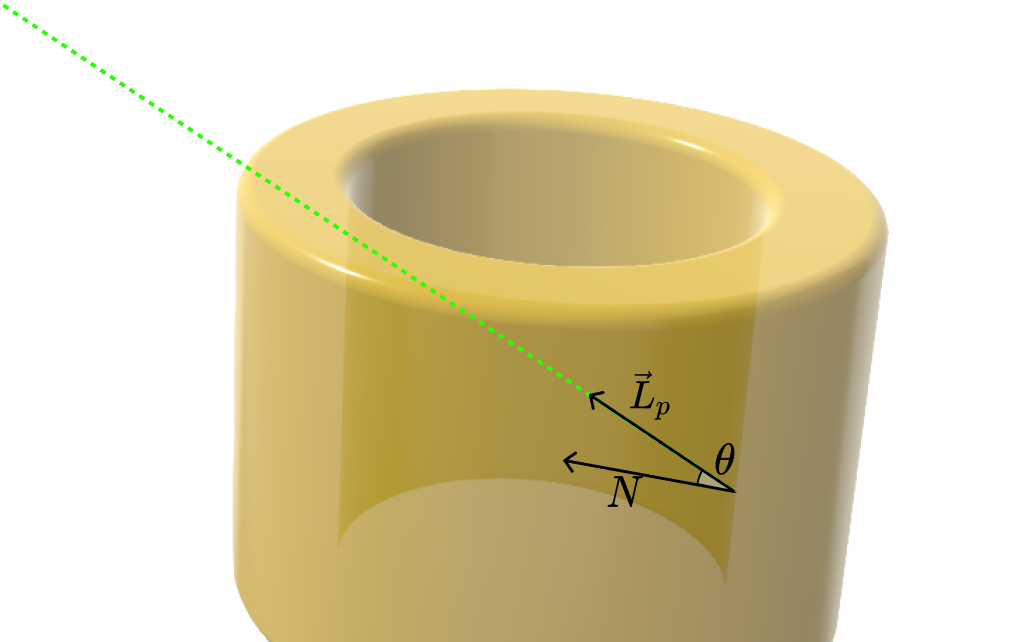
\includegraphics[scale = 0.3]{img/C8/no-convexo.png}
    \caption{Sombra en un objeto no convexo}
    \label{fig:objeto-no-convexo}
\end{figure}

La forma por tanto de saber si el punto está o no a la sombra es lanzar un rayo en la misma dirección que la luz y averiguar si existe alguna intersección con el fractal. En caso de que la haya multiplicamos por $0$ el valor de la componente difusa y la especular (el punto está a la sombra). Si no existe impacto se establece que la luz incide directamente sobre el punto y se multiplicarían por $1$ las componentes difusa y especular. Este proceso debe repetirse con cada una de las fuentes de luz que se utilicen.

Y para calcular si un rayo impacta o no con el fractal utilizamos ray-marching, por este motivo no ha sido posible hacer esta mejora antes. 

Necesitamos entonces una función que, dado un punto, trace un rayo en dirección de una fuente de luz dada y devuelva 0 si hay intersección con el fractal y 1 si no la hay. Fijémonos que las iteraciones de ray-marching deben comenzar a una pequeña distancia (mayor que $\varepsilon$) del punto que queremos evaluar, porque en caso de que este punto esté en el propio fractal y se comience a distancia $0$ el proceso finalizaría en la primera iteración y consideraría que todos los puntos del fractal están a la sombra, cosa que no tiene sentido. 

Para abreviar el código, llamamos en el siguiente código \verb|get_dist| a la SDF del objeto que se esté visualizando, la cual depende de la variable \verb|u_fractal|.
\begin{lstlisting}
float light_is_visible(Directional_light light, vec3 p) {
    Ray R;
    R.orig = p; R.dir = normalize(light.dir);
    float t = 2.0*u_epsilon;
    float h;
    // Ray Marching 
    for(int i = 0; i < 50; i++ ) {
        h=get_dist(ray_at(R,t));
        if(h < u_epsilon)
            return 0.0;
        t += h;
        if(t >= MAX_DIST) break;
    }
    return 1.0;
}
\end{lstlisting}

Y ahora debemos modificar la función que evalúa el modelo de iluminación, de forma que para cada luz direccional hace una llamada a \verb|light_is_visible| y multiplica el resultado por la componente difusa y la especular, de forma que si el punto está completamente a la sombra únicamente se sumaría la componente ambiental. En caso de que el punto esté en la sombra de una luz pero iluminado por otra se sumaría únicamente la componente ambiental de una pero también la difusa y especular de la otra. Por último, si está iluminado por las dos se evaluarían las tres componentes: ambiental, difusa y especular. 

\begin{lstlisting}
vec4 evaluate_lighting_model( Directional_light lights[ARRAY_TAM], 
    int num_lights, Hit_record hr ) {
    // ... 
    float visibility;
    vec4 L_in = vec4(0.0, 0.0, 0.0, 1.0);
    for(int i = 0; i < ARRAY_TAM; i++){
        if(i == num_lights) break;
        // ... 
        visibility = light_is_visible(light, hr.p);
        // ... 
        L_in += visibility * light.color 
                * (diffuse + specular);
    }
    L_in += ambient;
    return vec4(L_in.xyz, 1.0);
}
\end{lstlisting}

El resultado es el que se puede observar en la imagen \ref{fig:sombra-sin-suavizado}, donde podemos ver la sombra que provoca el conjunto de Julia $\mathcal{J}_{-0.12+0.75i}$ (que por cierto es la generalización 3D de la imagen \ref{fig:julia-explicados} (a)) sobre puntos de sí mismo y en puntos del plano.

\begin{figure} [ht]
    \centering
    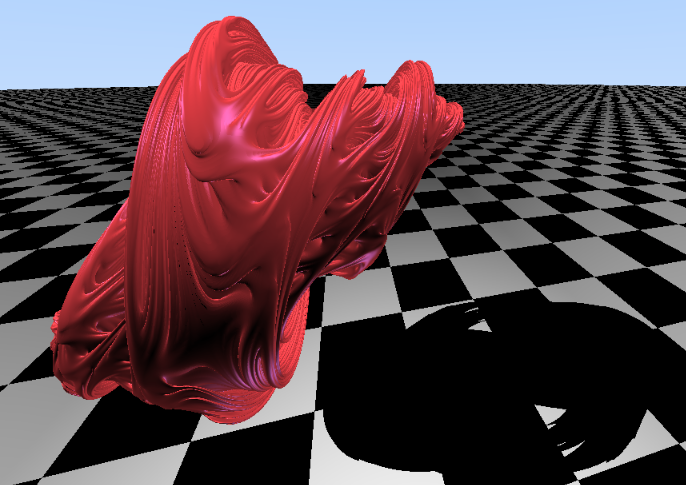
\includegraphics[scale = 0.45]{img/C8/sombra-1.png}
    \caption{Sombras arrojadas}
    \label{fig:sombra-sin-suavizado}
\end{figure}

Así conseguimos sombras arrojadas por todas las luces que tengamos. La manera más óptima y correcta que hemos conseguido de iluminar la escena es mediante dos luces direccionales blancas cuyos vectores de dirección son $(-1,1,0)$ y $(1,1,0)$, es decir, dos luces que iluminan `desde arriba y por ambos lados'. Sin embargo, esto provoca que la parte de abajo de los fractales siempre se vea oscura, por lo que hemos dotado a la escena de una tercera luz direccional en la dirección $(0,-1,0)$, con la particularidad de que esta no arroja sombras (siempre se le asigna \verb|visibility=1.0|), simplemente aporta iluminación a las partes bajas.

El resultado hasta ahora es bueno, pero aún así los límites de las sombras están muy marcados, lo cual queda poco realista. La apariencia mejoraría si se suavizaran los bordes, asignándole valores intermedios entre $0$ y $1$ a puntos que, aunque no estén en la sombra del conjunto, estén cerca. El truco consiste en pensar en los rayos que, aunque no impacten con el conjunto, pasen muy cerca de él. En estos casos pondríamos los puntos en cuestión en una especie de penumbra, de forma que cuanto más cerca pase del conjunto, más oscuro se representará, es decir, se devolverá un valor más cercano a $0$. Por tanto, calcularemos un factor de penumbra en cada iteración de ray-marching y nos quedaremos con el menor de ellos. Tan solo tenemos que añadir una línea de código a \verb|light_is_visible|.

\begin{lstlisting}
float light_is_visible(Directional_light light, vec3 p) {
    // ... 
    float res = 1.0; // Inicialmente 1
    float k = 16.0; // Constante de suavizado
    for(int i = 0; i < MAX_STEPS; i++ ) {
        h = get_dist(ray_at(R, t));
        if(h < u_epsilon)
            return 0.0;
        // Calculamos el nuevo factor de penumbra
        res = min(res, k*h/t); 
        t += h;
        if(t >= MAX_DIST) break;
    }
    return res;
}
\end{lstlisting}

La constante \verb|k| es un factor que indica si el suavizado es más o menos notable. El valor $16$ es suficientemente bueno para nuestro cometido, véase el resultado final en la imagen \ref{fig:sombras-final}, pero mostramos en las imágenes \ref{fig:sombras-k} la representación con los valores $k=2,32$. Nótese como en la imagen \ref{fig:sombras-k} (a) el sombreado es muy difuminado y en la imagen \ref{fig:sombras-k} (b) es bastante más marcado.

\begin{figure} [ht]
    \centering
    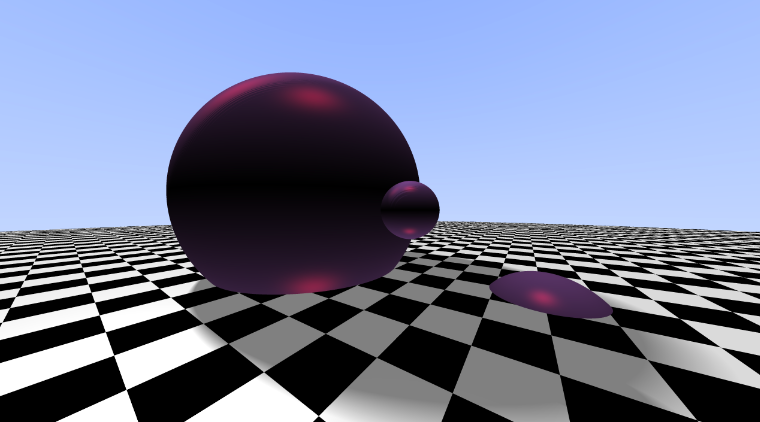
\includegraphics[scale = 0.45]{img/C8/sombras-final.png}
    \caption{Resultado final de la modificación}
    \label{fig:sombras-final}
\end{figure}


\begin{figure}[ht]
    \centering
    \begin{tabular}{cc}
        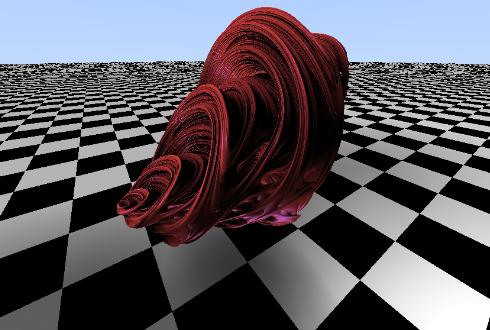
\includegraphics[scale=0.4]{img/C8/sombras-k-2.png} &
      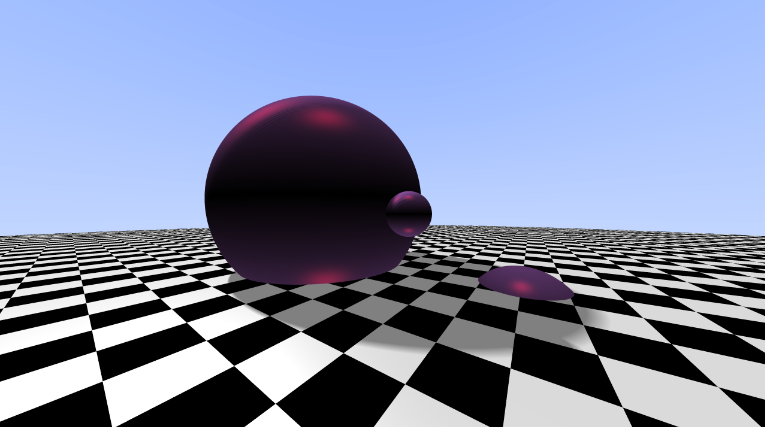
\includegraphics[scale=0.42]{img/C8/sombras-k-32.png} \\    
    (a) $k=2$ & (b) $k=32$  \\
    \end{tabular}
    \caption{Sombras con el parámetro $k=2,32$}
    \label{fig:sombras-k}
\end{figure}

Para apreciar de una forma más claro el efecto de la fuente de luz que ilumina la parte baja del fractal, presentamos en la imagen \ref{fig:desde-abajo} el conjunto de ejemplo que estamos utilizando en todas las imágenes de esta sección visto desde abajo, que gracias a la luz direccional cuya dirección es $(0,-1,0)$ se ve alumbrado.

\begin{figure} [ht]
    \centering
    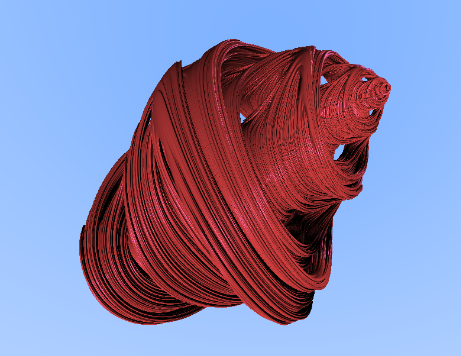
\includegraphics[scale = 0.45]{img/C8/desde-abajo.png}
    \caption{Conjunto de Julia visto desde abajo}
    \label{fig:desde-abajo}
\end{figure}

Para terminar esta sección y con el objetivo de añadir eficiencia e interactividad se ha añadido una variable \verb|uniform| de tipo \verb|bvec3|, es decir, una tripleta de booleanos, que sirve para especificar desde JavaScript qué luces queremos que proyecten sombras. Así podemos proyectar las sombras de la luz que queramos cuando busquemos realismo o desactivarlas cuando queramos mayor rapidez en la ejecución.

\begin{lstlisting}
uniform bvec3 u_shadows;
\end{lstlisting}


\subsection{Antiliasing}

El \textit{antiliasing} es una técnica que nos permite suavizar los bordes en las imágenes presentadas por píxeles. Para ello, debemos implementar algunos métodos concretos para que la imagen se presente más real. Por ejemplo, fíjese en la imagen \ref{fig:no-antiliasing}, en la cual se notan mucho los bordes entre las casillas negras y blancas, de forma que si ampliamos la imagen se vería muy pixelada.

\begin{figure} [ht]
    \centering
    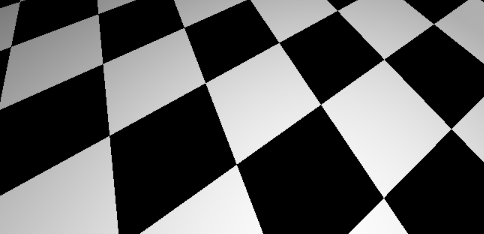
\includegraphics[scale = 0.5]{img/C8/no-antiliasing.png}
    \caption{Suelo antes de aplicar antiliasing}
    \label{fig:no-antiliasing}
\end{figure}

Para corregir este efecto, debemos tener en cuenta que al dividir el plano de proyección en píxeles lanzamos un único rayo por píxel, pero por la región del plano que corresponde puede pasar una recta diagonal como las de la imagen \ref{fig:no-antiliasing}, lo cual puede derivar en que un pixel se dibuje totalmente negro cuando realmente no lo es. De hecho podría ocurrir que en su mayoría el píxel fuera blanco pero justo el rayo se lanza hacia un punto que se evalúa como negro, en cuyo caso el píxel se colorearía negro. Fijémonos en la figura \ref{fig:pantalla-antiliasing} (a), en la cual representamos una pantalla de $5\times 3$ píxeles y cada punto señalado sería un punto del plano de proyección hacia el cual se lanzaría un rayo según las técnicas implementadas hasta el momento. La forma de solucionar este impedimento es lanzar más de un rayo por píxel, de forma que se cubra una región más representativa del mismo y se promedie el color que devuelve cada rayo en cada uno de los puntos. Para ello, fijamos un número natural $n\in\N$ y programaremos la forma de lanzar $n^2$ rayos en cada píxel, tal y como vemos en la imagen \ref{fig:pantalla-antiliasing} (b) con $n=2$.

\begin{figure}[ht]
    \centering
    \begin{tabular}{cc}
        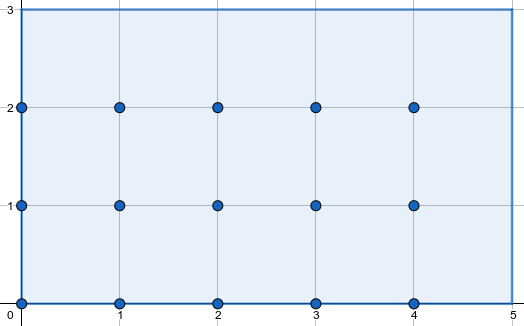
\includegraphics[scale=0.35]{img/C8/pixeles-sin-antiliasing.png} &
      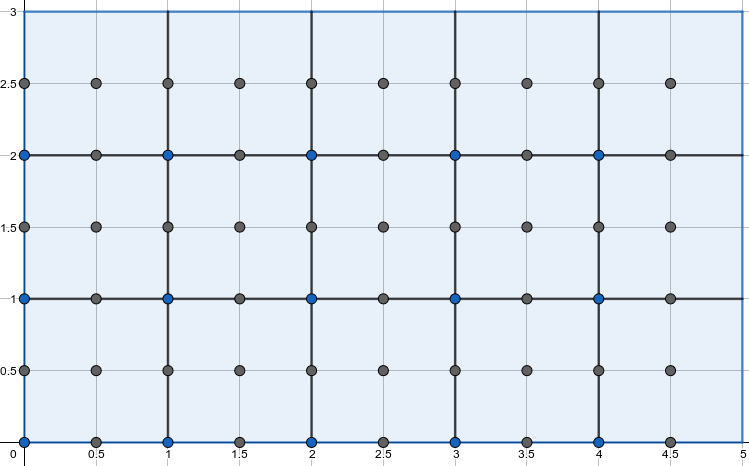
\includegraphics[scale=0.243]{img/C8/pixeles-con-antiliasing.png} \\    
    (a) Sin antiliasing & (b) Con antiliasing  \\
    \end{tabular}
    \caption{Representación de los rayos que se lanzan a una pantalla}
    \label{fig:pantalla-antiliasing}
\end{figure}

Por tanto, en \verb|main|, cuando obtenemos \verb|u,v| y creamos el rayo, debemos calcular $n^2$ coordenadas. Recordemos, de la sección \ref{section:camara}, \verb|u,v| son las coordenadas de dispositivo normalizadas en $[0,1]$, es decir:
\begin{lstlisting}
vec2 uv = gl_FragCoord.xy / vec2(image_width, image_height);
float u = uv.x;
float v = uv.y;
\end{lstlisting}

Por lo que ahora debemos sumarle a estas variables pequeños incrementos hasta completar el píxel. Concretamente, ahora dividimos el ancho de un píxel en $n$ intervalos, análogamente con el alto. Por tanto, el incremento sería de $h_w:=\frac{1}{image\_width\cdot n}$ en anchura y de $h_h:=\frac{1}{image\_height\cdot n}$ en altura. Pensemos que si normalizamos la pantalla a $[0,1]\times[0,1]$, entonces las dimensiones de un píxel son $\frac{1}{image\_width}\times\frac{1}{image\_height}$, y cada dimensión la queremos dividir en $n$, de ahí el valor del incremento.

Seguidamente, creamos un array de colores, el cual tendrá $n^2$ elementos, uno por cada rayo que lancemos. Por cada posición del array calculamos la coordenada de dispositivo normalizada del punto al cual queremos lanzar el rayo, llamamos a \verb|get_ray|, a \verb|ray_color| y almacenamos el valor de retorno de esta última en el array. Finalmente calculamos la media de todos los colores del array y ese es el valor que finalmente devolvemos. 

La forma de, a partir del índice $i$ del array, obtener la coordenada correspondiente es imaginar que lo dividimos en $n$ grupos de $n$ componentes cada uno. Cada grupo representa una fila de puntos del píxel. Por tanto, aplicando la división entera, $i/n$ será la fila e $i\%n$ la columna. Por lo que habría que sumar $(i/n)h_w$ a la coordenada anchura inicial e $(i\%n)h_h$ a la altua para obtener la coordenada a la que lanzar el rayo.

El código por tanto sería el siguiente

\begin{lstlisting}
// Antiliasing
vec2 uv = gl_FragCoord.xy / vec2(image_width, image_height);
float u,v;
int nSamples = 3;  // O cualquier valor
float hw = 1.0 / (float(image_width * nSamples)),
      hh = 1.0 / (float(image_height * nSamples));
Ray r;
vec4 colors[ARRAY_TAM]; 
for(int i = 0; i < ARRAY_TAM; i++) {
    if(i == nSamples*nSamples) break;
    int x =  i/nSamples;
    int y =  i - nSamples*x;
    u = uv.x + float(x) * hw;
    v = uv.y + float(y) * hh;
    r = get_ray(cam, u, v);
    colors[i] = ray_color(r, ground, lights, num_lights);
}
gl_FragColor = color_array_average(colors, nSamples*nSamples);
\end{lstlisting}
Donde la función \verb|color_array_average|, tal y como su nombre indica, calcula la media de un array de colores.

Con esta modificación y fijando el valor que consideremos en \verb|nSamples| se consiguen resultados como el de la figura \ref{fig:antiliasing}. Como se puede ver, los bordes son más suaves y de mejor calidad

\begin{figure} [ht]
    \centering
    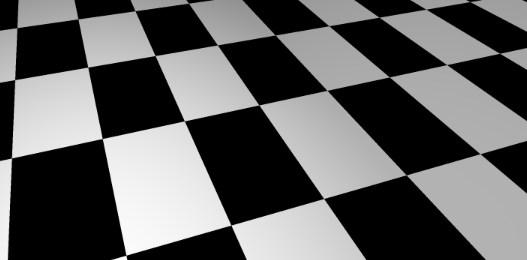
\includegraphics[scale = 0.5]{img/C8/antiliasing.png}
    \caption{Suelo tras de aplicar antiliasing}
    \label{fig:antiliasing}
\end{figure}

El principal y mayor inconveniente que presenta esta técnica es que, como se puede imaginar, es $n^2$ veces más costosa que lanzar un único rayo por píxel, por lo que ralentiza muchísimo la ejecución, comprometiendo incluso la posibilidad de hacer ejecuciones en tiempo real. Sin embargo, si se desea una imagen concreta con parámetros muy claros y no tanto la interacción es una buena herramienta, pues proporciona un nivel de detalle mucho mayor incluso para valores de $\varepsilon$ muy pequeños, fíjese por ejemplo en la representación de la imagen \ref{fig:julia-antiliasing}, la cual tiene una gran calidad y un alto nivel de detalle a pesar de haber usado $\varepsilon=10^{-5}$.

\begin{figure} [ht]
    \centering
    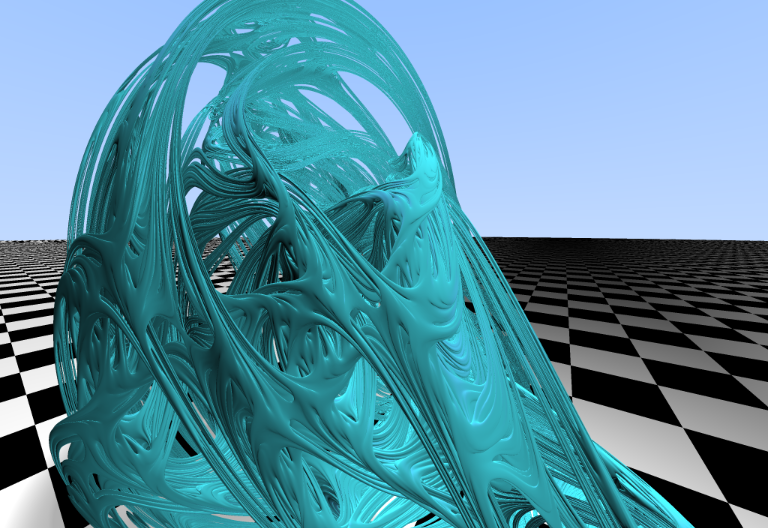
\includegraphics[scale = 0.4]{img/C8/julia-antiliasing.png}
    \caption{Conjunto de Julia aplicando antiliasing}
    \label{fig:julia-antiliasing}
\end{figure}

Precisamente por este costo, se incluye la posibilidad de decidir si se desea o no aplicar antiliasing, y en caso afirmativo, cuántos rayos por píxel se desean trazar. Esto se consigue mediante una variable \verb|uniform| booleana que en caso de valer \verb|true| se ejecutaría el código del antiliasing y en caso contrario se ejecutaría el código normal con un rayo por píxel. El primero obviamente es más ligero y favorece la fluidez, pero el segundo ofrece mejores resultados a cambio de sacrificar dicha fluidez.

\begin{lstlisting}
    uniform bool u_antiliasing;
    uniform int u_nSamples;
// ...
void main() {
    // ... 
    if(u_antiliasing) {
        // Antiliasing
        int nSamples = u_nSamples;
        // ... 
    }
    else {
        // No antiliasing
        // ...
    }
}   
\end{lstlisting}

\section{Posibles optimizaciones}

El software, en lo que a funcionalidad se refiere está completo, sin embargo puede ser lento en algunos dispositivos dependiendo de la GPU que posean. En gran medida, lo que más ralentiza la ejecución es el hecho de evaluar la SDF correspondiente en cada iteración del ray-marching, ya que esto supone iterar el punto y aplicar transformaciones como el logaritmo que son más costosas. Por lo que trataremos de introducir algunas medidas que nos permitan ahorrarnos algunas ejecuciones de las SDFs, todas ellas basadas en una misma idea: las esferas englobantes.

\subsection{Esferas englobantes}
 
Si se lanza un rayo que está muy lejano al conjunto que se esté visualizando o que apunta directamente al cielo o al suelo, antes de converger al suelo o diverger al cielo hay que evaluar, sobre todo en este último caso, hasta mil veces la SDF cuando realmente casi desde el principio podría saberse que no va a intersecar al conjunto. Para ahorrarnos todas estas evaluaciones podemos utilizar lo que se denominan esferas englobantes (\textit{bounding spheres}).

La técnica consiste en crear una esfera que `englobe' el conjunto, en el sentido de que éste quepa completamente en el interior de la misma. Antes de aplicar ray-marching, reutilizaríamos el código que ya programamos en la sección \ref{subsection:esfera} para calcular analíticamente la intersección de un rayo con una esfera, aunque esta vez sólo nos interesa saber si el rayo interseca la esfera englobante, no el punto ni el valor de $t$. Si se calcula que el rayo no golpea la esfera englobante, entonces no se calcula la distancia al conjunto en ninguna iteración, pues sabemos que no habrá intersección con el mismo, aunque aún puede haber intersección con el plano, pero al no tener que calcular la SDF del conjunto que se esté visualizando la ejecución es mucho más rápida.

Para implementar este método, hemos probado empíricamente qué radio de esfera se ajusta mejor a los conjuntos de Julia, al conjunto de Mandelbrot y al conjunto de Mandelbub, obteniendo respectivamente $2.5$, $2$ y $1.5$ respectivamente. Por tanto, ajustamos el radio de esta esfera y sólo calculamos las SDFs en caso de impacto.

\begin{lstlisting}
// Returns true if R hits S, false otherwise
bool hit_sphere_limits( Sphere S, Ray R ){
    vec3 oc = R.orig - S.center;
    float a = dot(R.dir,R.dir);
    float b = 2.0 * dot(oc, R.dir);
	float c = dot(oc,oc) - S.radius*S.radius;
    float discriminant = b*b - 4.0*a*c;
    return discriminant >= 0.0;
}

vec4 ray_color(Ray r, ...) {
    // ... 
    Sphere bounding_sphere;
    bounding_sphere.center = vec3(0.0, 0.0, 0.0);
    bounding_sphere.radius = u_fractal == 1 ? 1.5 : 
        (u_fractal == 2 ? 2.5 : 2.0);
    bool hits_bounding_sphere = hit_sphere_limits(bounding_sphere, r);
    
    // Ray Marching
    for(int i = 0; i < MAX_STEPS; i++) {
        // Distancia al plano ... 
        // ... 
        // Distancia Julia/Mandelbrot/Mandelbub
        if(hits_bounding_sphere) {
            dist = get_dist(p)
            // ... 
        }
        // ... 
    }
    // ...
}
\end{lstlisting}

Y con esta simple técnica podemos optimizar bastante las escenas en las que el fractal aparece más lejano. Sin embargo, si queremos ampliar detalles del conjunto no influiría, pues la gran mayoría de los rayos impactan con la esfera englobante. Aún así, en caso de estar cerca las iteraciones que se dan representan un número pequeño, así que mejoramos el rendimiento de una u otra forma.

\subsection{Optimización de sombras con esferas englobantes}

En ciertos píxeles hay que aplicar varias veces ray-marching, es el caso de los píxeles que corresponden a puntos del fractal o del plano que consideramos como suelo, ya que como se ha explicado en la sección \ref{subsection:sombras}, la forma de añadir sombras a la escena es, a partir del punto donde se produce la intersección con el rayo, aplicar ray-marching en la dirección de cada una de las fuentes de luz y buscar posibles intersecciones con el conjunto que se visualice en la escena, asignando así a cada fuente un coeficiente de visibilidad. Aplicar varias veces ray-marching implica muchas ejecuciones de las SDFs, lo cual también ralentiza la ejecución. 

Sin embargo, al igual que con el ray-marching principal de \verb|ray_color|, podemos desde el principio descartar todos los rayos que no intersequen la esfera englobante. Esta mejora se puede hacer con una ligera modificación del método \verb|light_is_visible|.

\begin{lstlisting}
float light_is_visible(Directional_light light, vec3 p) {
    Ray R;
    R.dir = normalize(light.dir);
    R.orig = p;
    // ... 
    if(!hit_sphere_limits(bounding_sphere, R))
        return 1.0;
    // Ray Marching
    for(int i = 0; i < 50; i++ ) {
        // ... 
    }
    return res;
}
\end{lstlisting}

El inconveniente es que esta mejora sólo puede aplicarse a ocasiones en las que el canvas visualice puntos lejanos al conjunto, por lo que cuando se esté graficando un detalle de un fractal puede ser poco útil. No obstante, en estos casos al haber menos puntos del plano directamente no tiene por qué ejecutarse en gran medida el código correspondiente a las sombras, por lo que hemos mejorado la eficiencia en los casos donde se ejecutaba dicho código más veces, es decir, en planos más abiertos y lejanos al conjunto.

